\documentclass[12pt,a4paper]{report}

\usepackage{styles/dolgozat}

\usepackage{listings}
%\usepackage{styles/cpp}

\usepackage{tikz}
\usetikzlibrary{positioning}

\usepackage{hyperref}

\usepackage{tcolorbox}
\tcbuselibrary{listings,skins}

\newtcblisting{tikzcode}{
	tikz lower=,
	listing side text,
	bicolor,
	colback=lightgray!30,
	colbacklower=white,
	colframe=lightgray!30,
	righthand width=3cm
}

\lstdefinestyle{latex}{language=[LaTeX]TeX}

\begin{document}

\pagestyle{empty} %a címlapon ne legyen semmi=empty, azaz nincs fejléc és lábléc

% A Miskolci Egyetem címere
{\large
\begin{center}
\vglue 1truecm
\textbf{\huge\textsc{Szakdolgozat}}\\
\vglue 1truecm

\includegraphics[width=4.8truecm, height=4truecm]{images/me_logo.png}\\
\textbf{\textsc{Miskolci Egyetem}}
\end{center}}

\vglue 1.5truecm %függõleges helykihagyás

% A szakdolgozat címe, akár több sorban is
{\LARGE
\begin{center}
\textbf{Online grafikus szerkesztő alkalmazás \\ TikZ ábrák készítéséhez}
\end{center}}

\vspace*{2.5truecm}
% A hallgató neve, évfolyam, szak(ok), a konzulens(ek) neve
{\large
\begin{center}
\begin{tabular}{c}
\textbf{Készítette:}\\
Veréb Tamás\\
Programtervező informatikus
\end{tabular}
\end{center}
\begin{center}
\begin{tabular}{c}
\textbf{Témavezető:}\\
Vadon Viktória
\end{tabular}
\end{center}}
\vfill
% Keltezés: Hely, év
{\large
\begin{center}
\textbf{\textsc{Miskolc, 2021}}
\end{center}}

\newpage


\newpage

\pagestyle{empty}

%Feladatkiiras
\begin{flushleft}
\textsc{\bfseries Miskolci Egyetem}\\
Gépészmérnöki és Informatikai Kar\\
Alkalmazott Matematikai Intézeti Tanszék\hspace*{4cm}\hfil \textbf{Szám:}
\end{flushleft}
\vskip 0.5cm
\begin{center}
\large\textsc{\bfseries Szakdolgozat Feladat}
\end{center}
\vskip 0.5cm
Veréb Tamás (HQYII1) programtervező informatikus jelölt részére.\newline

\noindent\textbf{A szakdolgozat tárgyköre:} latex, tikz\newline

\noindent\textbf{A szakdolgozat címe:} Online grafikus szerkesztő alkalmazás TikZ ábrák készítéséhez\newline

\noindent\textbf{A feladat részletezése:}

\medskip

\emph{A TikZ egy LaTeX-hez készített csomag, amely segítségével vektorgrafikus ábrákat lehet készíteni. Az előre definiált rajzelemek paramétereinek a megadásával procedurális módon lehet vele rajzolni többek között például gráfokat, grafikonokat, geometriához kapcsolódó illusztrációkat.}

\medskip

\emph{A csomag a rajzolási műveletek megadását szöveges formában teszi lehetővé. A dolgozat célja, hogy bemutassa egy online szerkesztőfelületnek a tervezését és elkészítését, amely grafikus szerkesztést tesz lehetővé, az eredményt pedig LaTeX-be visszailleszthető forrásszöveg formájában adja.}

\medskip

\emph{A dolgozat felsorolja a hasonló célú alkalmazásokat, összehasonlítja azok funkcióit. Specifikálja a szerkesztőfelületet. Vizsgálja annak lehetőségét, hogy a korábban már szerkesztett ábrák milyen esetekben módosíthatók az alkalmazással a LaTeX-es forráskód ismeretében.}

\vfill

\noindent\textbf{Témavezető:} Vadon Viktória (egyetemi tanársegéd) \newline

% \noindent\textbf{Konzulens(ek):} (akkor kötelezõ, ha a témavezetõ nem valamelyik matematikai tanszékrõl való; de persze lehet egyébként is)\newline

\noindent\textbf{A feladat kiadásának ideje:} \newline

%\noindent\textbf{A feladat beadásának határideje:}

\vskip 2cm

\hbox to \hsize{\hfil{\hbox to 6cm {\dotfill}\hbox to 1cm{}}}

\hbox to \hsize{\hfil\hbox to 3cm {szakfelelős}\hbox to 2cm{}}

\newpage

\vspace*{1cm}  
\begin{center}
\large\textsc{\bfseries Eredetiségi Nyilatkozat}
\end{center}
\vspace*{2cm}  

Alulírott \textbf{Veréb Tamás}; Neptun-kód: \texttt{HQYII1} a Miskolci Egyetem Gépészmérnöki és Informatikai Karának végzős Programtervező informatikus szakos hallgatója ezennel büntetőjogi és fegyelmi felelősségem tudatában nyilatkozom és aláírásommal igazolom, hogy \textit{Online grafikus szerkesztő alkalmazás TikZ ábrák készítéséhez}
című szakdolgozatom saját, önálló munkám; az abban hivatkozott szakirodalom
felhasználása a forráskezelés szabályai szerint történt.\\

Tudomásul veszem, hogy szakdolgozat esetén plágiumnak számít:
\begin{itemize}
\item szószerinti idézet közlése idézőjel és hivatkozás megjelölése nélkül;
\item tartalmi idézet hivatkozás megjelölése nélkül;
\item más publikált gondolatainak saját gondolatként való feltüntetése.
\end{itemize}

Alulírott kijelentem, hogy a plágium fogalmát megismertem, és tudomásul veszem, hogy
plágium esetén szakdolgozatom visszautasításra kerül.

\vspace*{3cm}

\noindent Miskolc, \hbox to 2cm{\dotfill} .év \hbox to 2cm{\dotfill} .hó \hbox to 2cm{\dotfill} .nap

\vspace*{3cm}

\hspace*{8cm}\begin{tabular}{c}
\hbox to 6cm{\dotfill}\\
Hallgató
\end{tabular}



\newpage

\noindent 1.

\begin{tabular}{cl}
&szükséges (módosítás külön lapon) \\
A szakdolgozat feladat módosítása& \\
& nem szükséges\\
&\\
\hbox to 4cm{\dotfill}&\multicolumn{1}{c}{\hbox to 5cm{\dotfill}}\\
dátum& \multicolumn{1}{c}{témavezető(k)}
\end{tabular}
\vskip1.5mm

\noindent 2. A feladat kidolgozását ellenőriztem:

\vskip1.5mm

\begin{tabular}{l@{\hspace*{4cm}}l}
témavezető (dátum, aláírás):& konzulens (dátum, aláírás):\\
\dotfill&\dotfill\\
\dotfill&\dotfill\\
\dotfill&\dotfill
\end{tabular}

\vskip1.5mm

\noindent 3. A szakdolgozat beadható:

\vskip1.5mm

\begin{tabular}{@{\hspace*{1.3cm}}c@{\hspace*{2.1cm}}c}
\hbox to 4cm{\dotfill}&\multicolumn{1}{c}{\hbox to 5cm{\dotfill}}\\
dátum& \multicolumn{1}{c}{témavezető(k)}
\end{tabular}

\vskip1.5mm

\noindent 4.
\begin{tabular}[t]{@{}l@{\hspace*{1mm}}l@{\hspace*{1mm}}l@{}}
A szakdolgozat& \hbox to 3.5cm{\dotfill} &szövegoldalt\\
              & \hbox to 3.5cm{\dotfill} &program protokollt (listát, felhasználói leírást)\\
              &\hbox to 3.5cm{\dotfill}   &elektronikus adathordozót (részletezve)\\
              &\hbox to 3.5cm{\dotfill} & \\
              &\hbox to 3.5cm{\dotfill} &egyéb mellékletet (részletezve)\\
              &\hbox to 3.5cm{\dotfill} &\\
\end{tabular}
\newline tartalmaz.

\vskip1.5mm

\begin{tabular}{@{\hspace*{1.3cm}}c@{\hspace*{2.1cm}}c}
\hbox to 4cm{\dotfill}&\multicolumn{1}{c}{\hbox to 5cm{\dotfill}}\\
dátum& \multicolumn{1}{c}{témavezető(k)}
\end{tabular}

\noindent 5.

\begin{tabular}{ll}
&bocsátható\\
A szakdolgozat bírálatra& \\
& nem bocsátható\\
\end{tabular}

\vskip1.5mm

\noindent A bíráló neve: \hbox to 8cm{\dotfill}

\vskip4mm

\begin{tabular}{@{\hspace*{1.3cm}}c@{\hspace*{2.1cm}}c}
\hbox to 4cm{\dotfill}&\multicolumn{1}{c}{\hbox to 5cm{\dotfill}}\\
dátum& \multicolumn{1}{c}{szakfelelős}
\end{tabular}

\noindent 6.
\begin{tabular}[t]{@{}l@{\hspace*{1mm}}l@{\hspace*{1mm}}l@{}}
A szakdolgozat osztályzata& &\\
&a témavezető javaslata:& \hbox to 3cm{\dotfill}\\
&a bíráló javaslata:& \hbox to 3cm{\dotfill}\\
&a szakdolgozat végleges eredménye:& \hbox to 3cm{\dotfill}
\end{tabular}

\vspace*{4mm}

\noindent Miskolc, \hbox to 4.5cm{\dotfill} \hspace*{2.5cm}
\begin{tabular}[t]{cc}
\hbox to 6cm{\dotfill}\\
a Záróvizsga Bizottság Elnöke
\end{tabular}


\cleardoublepage
\pagenumbering{gobble}
\tableofcontents
\cleardoublepage
\pagenumbering{arabic}

\newpage

\pagestyle{fancy}

\Chapter{Bevezetés}

A szakdolgozatom egy online grafikus szerkesztő elkészítése és dokumentálása. A szerkesztő a \textit{TikZ} \LaTeX\ csomag nyelvi elemeire épül. A webes fejlesztés miatt a HTML5 és a JavaScript nyelv adja az alapokat. A rajzolási felületet a \textit{p5.js} nyújtja.

A \LaTeX\ -et széles körben használják a tudományos életben tudományos dokumentumok közlésére és közzétételére számos területen, többek között a matematikában, az informatikában, a mérnöki tudományokban, a fizikában, a kémiában, a közgazdaságtanban, a nyelvészetben, a kvantitatív pszichológiában, a filozófiában és a politikatudományban. A \LaTeX\ a \TeX\ szövegszerkesztő programot használja a kimenet formázásához, és maga is a \TeX\ makrónyelvben íródott.

A tanulmányaim során megismerkedtem a JavaScript nyelvvel és egy könnyen elsajátítható programozási nyelvnek találtam. A JavaScript, gyakran JS rövidítéssel, az ECMAScript specifikációnak megfelelő programozási nyelv. A JavaScript magas szintű, gyakran futásidejű fordítású nyelv. Az ECMAScript 2015 (\textit{ES6}) bevezetésével egy jól használható  objektumorientált nyelv lett.

A következő oldalakban megismerkedhetünk a TikZ csomag telepítésével, a grafikus elemivel, valamint a már meglévő szerkesztők kerülnek jellemzésre, majd összehasonlításra különböző szempontok alapján. Ezek a feltételek kerülnek megfogalmazásra a készülő alkalmazással szemben, mint követelmények.

 A következő szegmens már a dokumentáció része az alkalmazásnak. Itt kerülnek kifejtésre a felhasznált függvénykönyvtárak, az elkészült alkalmazás felépítése, funkciói, használata, és a definiált osztályok leírása, a \textit{TikZ}, mint \LaTeX\ könyvtár és a \textit{p5.js}, mint JavaScript függvénykönyvtár eszközkészletében található eltérések. 
 
 A továbbiakban már az elkészült alkalmazással megvalósított ábrák kerülnek bemutatásra.


\Chapter{A TikZ és eszközkészlete}

% Kb. 8 oldal

\Section{Ábrák szerkesztése LaTeX-ben}

A rajzolás megkönnyítése érdekében a TikZ-t használjuk, amely egy frontend réteg a PGF-hez. Egy ábrát létrehozni azt jelenti, hogy egyenes vagy görbe vonalak sorozatát rajzoljuk meg. A TikZ parancsaira és szintaxisára olyan források voltak hatással, mint a METAFONT, a PSTricks és még sokan mások.

\noindent
A pontok és koordináták megadására a TikZ egy speciális szintaxist biztosít. A legegyszerűbb, ha kerek zárójelben vesszővel elválasztott két dimenziót használunk, például (4pt, 6pt). Ha az egység nincs megadva, akkor az xy-koordináta rendszerének alapértelmezett értékeit használjuk. Ez azt jelenti, hogy az egységnyi x-vektor 1 cm-rel jobbra, az egységnyi y-vektor pedig 1 cm-rel felfelé halad. 

\Section{A TikZ elemei}

\SubSection{Használata}
% usepackage, telepítés, útmutatók

Először is be kell állítanunk a környezetünket. Kezdetnek a következőképpen állítjuk be a fájlunkat:

\begin{lstlisting}[style=latex]
\documentclass{article}
\usepackage{tikz}
\begin{document}
	<content>
\end{document}
\end{lstlisting}

\noindent
Ezután kezdjük el az ábrák létrehozását. 


\SubSection{Szintaxis}
% Alapvető nyelvi elemek bemutatása

A szabály az, hogy minden TikZ grafikus rajzoló parancsnak a \lstinline{\tikz} parancs argumentumaként vagy a {tikzpicture} környezeten belül kell előfordulnia. 

\noindent
A {tikzpicture} környezet \LaTeX\ változata a következő:

\begin{lstlisting}[style=latex]
\begin{tikzpicture}[options]
	<content>
\end{tikzpicture}
\end{lstlisting}


\noindent
A környezeten belül megadott összes opció a teljes képre vonatkozik.

\noindent
A TikZ-ben minden ábra alapvető építőeleme a vonal. Egy vonalat a kezdőpont koordinátáinak megadásával kezdünk, mint például (0,0), majd hozzáadunk egy vonal bővítő műveletet, a legegyszerűbb csak "\lstinline{--}". A műveletet ezután a következő koordináta követi. Minden útvonalnak pontosvesszővel kell végződnie. Az vonal megrajzolásához a \lstinline{\draw} parancsot használjuk.

\noindent
Például a (0,0), (0,1), (1,0) pontok közötti háromszög megrajzolásához azt írhatjuk, hogy:

\begin{lstlisting}[style=latex]
\tikz\draw (0,0) -- (0,1) -- (1,0) -- (0,0);
\end{lstlisting}
vagy

\begin{lstlisting}[style=latex]
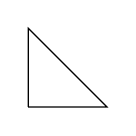
\begin{tikzpicture}
	\draw (0,0) -- (0,1) -- (1,0) -- (0,0);
\end{tikzpicture}
\end{lstlisting}


\begin{tikzcode}
\draw (0,0) -- (0,1) -- (1,0) -- (0,0);
\end{tikzcode}



\SubSection{Elérhető diagram elemek}
% Csomópontok, vonalak, feliratok, ívek, ...
% Ide kerülhetnek külön ábrák részletes magyarázatokkal (ténylegesen TikZ-s ábrák itt is).

A körök és ellipszisek rajzolásához a \textit{circle} és \textit{ellipse} műveletet használhatjuk. A kör műveletet egy sugár követi kerek zárójelben, míg az ellipszis műveletet kettő követi, egy az x-irányra és egy az y-irányra vonatkozóan, amelyeket az \textit{and} taggal választunk el, és kerek zárójelben helyezünk el. 

\begin{tikzcode}
\draw (0,0) ellipse (1 and 0.5);
\end{tikzcode}

\begin{tikzcode}
\draw (0,0) ellipse (0.5 and 1);
\end{tikzcode}

\noindent
A rácsháló (\textit{grid}), téglalap (\textit{rectangle}), a parabola (\textit{parabola}), és az ív (\textit{arc}) rajzolásához is hasonló műveletek is rendelkezésünkre áll. Az alábbiak példák ezen konstrukciók használatára:

\begin{tikzcode}
\draw (-1,-1) grid (1,1);
\end{tikzcode}

\begin{tikzcode}
\draw (-1,0) -- (1,0);
\draw (0,-1) -- (0,1);
\draw (0,0) circle (1);
\draw (-1,-1) rectangle (1,1);
\draw (-1,-1) parabola (1,1);
\end{tikzcode}

\noindent
Az ív hasznos egy szög ívének megrajzolásához. Megrajzolja a kör adott sugarú részét a megadott szögek között. Ezt a műveletet egy kerek zárójelben lévő hármasnak kell követnie. Az adattagokat kettőspontok választják el egymástól. Az első és a második a kör fokai, a harmadik pedig a sugara. Például a (\textit{30 : 160 : 2cm}) azt jelenti, hogy egy 2 cm sugarú körön 30 és 100 fok közötti ív lesz.

\begin{tikzcode}
\draw (0,0) arc (30:100:2cm);
\end{tikzcode}

\noindent
Az elemek elforgatásához vagy skálázásához egy \textit{rotate} vagy \textit{scale} opciót is hozzáadhatunk, akár egyszerre is a két lehetőséget.

\begin{tikzcode}
\draw[rotate=45] 
	(0,0) ellipse (1 and 0.5);
\end{tikzcode}

\begin{tikzcode}
\draw[scale=1.5] 
	(0,0) ellipse (1 and 0.5);
\end{tikzcode}

\begin{tikzcode}
\draw[rotate=45, scale=1.5] 
	(0,0) ellipse (1 and 0.5);
\end{tikzcode}

\noindent
A \textit{definecolor} paranccsal definiálhatunk és használhatunk színeket az alábbiak szerint:
\begin{tikzcode}
\definecolor{myrgb}{rgb}{1,0.2,0.3}
\definecolor{myRGB}{RGB}{255,51,76}
\draw [myrgb] (0,0.5) -- (1,0.5);
\draw [myRGB] (0,0) -- (1,0);
\end{tikzcode}

\noindent
A következő színeket érhetjük el bármiféle definiálás nélkül: 
\textit{white} (\tikz\draw (0,0) rectangle (0.5,0.25);),
\textit{lightgray} (\tikz\fill [lightgray](0,0) rectangle (0.5,0.25);),
\textit{gray} (\tikz\fill [gray](0,0) rectangle (0.5,0.25);),
\textit{darkgray} (\tikz\fill [darkgray](0,0) rectangle (0.5,0.25);),
\textit{black} (\tikz\fill [black](0,0) rectangle (0.5,0.25);),
\textit{red} (\tikz\fill [red](0,0) rectangle (0.5,0.25);),
\textit{violet} (\tikz\fill [violet](0,0) rectangle (0.5,0.25);),
\textit{purple} (\tikz\fill [purple](0,0) rectangle (0.5,0.25);),
\textit{magenta} (\tikz\fill [magenta](0,0) rectangle (0.5,0.25);),
\textit{pink} (\tikz\fill [pink](0,0) rectangle (0.5,0.25);),
\textit{green} (\tikz\fill [green](0,0) rectangle (0.5,0.25);),
\textit{lime} (\tikz\fill [lime](0,0) rectangle (0.5,0.25);),
\textit{olive} (\tikz\fill [olive](0,0) rectangle (0.5,0.25);),
\textit{brown} (\tikz\fill [brown](0,0) rectangle (0.5,0.25);),
\textit{orange} (\tikz\fill [orange](0,0) rectangle (0.5,0.25);),
\textit{yellow} (\tikz\fill [yellow](0,0) rectangle (0.5,0.25);),
\textit{blue} (\tikz\fill [blue](0,0) rectangle (0.5,0.25);),
\textit{cyan} (\tikz\fill [cyan](0,0) rectangle (0.5,0.25);),
\textit{teal} (\tikz\fill [teal](0,0) rectangle (0.5,0.25);).


\noindent
A \textit{fill} paranccsal kitölthetjük a megadott színnel a bármely zárt görbe által határolt tartományt. Az aktuális rajzolt görbe lezárásához használhatjuk a \lstinline{-- cycle} parancsot. A szín argumentumhoz használhatjuk a szín nevét, például \textit{green} (\tikz\fill [green](0,0) rectangle (0.5,0.25);), \textit{white} (\tikz\draw (0,0) rectangle (0.5,0.25);) és \textit{red} (\tikz\fill [red](0,0) rectangle (0.5,0.25);), vagy keverhetjük a színeket, mint a \textit{red!40!white}, ami azt jelenti, hogy 40\% pirosat és 60\% fehéret fogunk keverni.

\begin{tikzcode}
\fill[red!40!white] 
	(0,0) -- (0,1) -- (1,0) -- cycle;
\end{tikzcode}

\noindent
A kitöltést meg lehet adni egyszerűen a \textit{draw} parancs paramétereként is, ám ilyenkor a körvonal is rajzolva lesz:

\begin{tikzcode}
\draw[fill=red!40!white] 
	(0,0) -- (0,1) -- (1,0) -- cycle;
\end{tikzcode}

\noindent
Ez a színmegadás egyérteműen használható a körvonal szinének módosítására is:

\begin{tikzcode}
\draw[draw=green, fill=red!40!white] 
	(0,0) -- (0,1) -- (1,0) -- cycle;
\end{tikzcode}

\noindent
A vonalakat végpontjait testreszabhatjuk, így nyilakat hozhatunk létre:

\begin{tikzcode}
\draw [->] (0,1) -- (1,1);
\draw [<-] (0,0.5) -- (1,0.5);
\draw [|-|] (0,0) -- (1,0);
\end{tikzcode}

\noindent
A nyílhegyek esetében is rengeteg lehetséges opció van, a két végponton lévő nyílhegy szabadon variálható, egy pár ezek közül:
\begin{tikzcode}
\draw [stealth-stealth reversed] (0,1.5) -- (1,1.5);
\draw [to-to reversed] (0,1) -- (1,1);
\draw [latex-latex reversed] (0,0.5) -- (1,0.5);
\draw [|-|] (0,0) -- (1,0);
\end{tikzcode}

\noindent
Az \textit{arrows.meta} library további nyílhegyeket tartalmaz, ebből két darabot emelnék ki, melyek jól használhatók a fentiekkel kombinálva:

\begin{tikzcode}
\draw [{Stealth[open]}-stealth reversed] 
	(0,0.5) -- (1,0.5);
\draw [{Latex[open]}-latex reversed] (0,0) -- (1,0);
\end{tikzcode}

\noindent
Ha több szegmenst rajzolunk, a nyilak az első és az utolsó szegmens végpontjainál helyezkednek el. Ez többek között a tengelyek rajzolásához kényelmes:

\begin{tikzcode}
\draw [<->] (0,1) -- (0,0) -- (1,0);
\end{tikzcode}

\noindent
Ha a vonal vastagságát akarjuk módosítani, akkor szintén hasonlóképpen járhatunk el:

\begin{tikzcode}
\draw [thin] (0,1) -- (1,1);
\draw [thick] (0,0.5) -- (1,0.5);	
\draw [ultra thick] (0,0) -- (1,0);
\end{tikzcode}


\noindent
Ahhoz, hogy szöveget adjunk a képhez, csomópontot kell hozzáadnunk az útvonalhoz, mint a következőben:

\begin{tikzcode}
\draw 
	(1,1) node[circle,draw]{A} 
	-- 
	(2,2) node[circle,draw]{B};	
\end{tikzcode}

\noindent
A csomópontok az útvonal aktuális pozíciójába kerülnek, a [\textit{circle,draw}] opció a szöveget egy körrel veszi körül, amely az aktuális pozícióba rajzolódik.
Néha azt szeretnénk, ha a csomópont az aktuális koordináta jobb oldalán vagy fölött lenne. Ehhez viszont már szükséges a \textit{positioning} library hozzáadása is a fájlunkhoz.

\begin{tikzcode}
\draw 
(1,1) node[anchor=north east, circle, draw]{A} 
	-- 
(2,2) node[anchor=south west, circle, draw]{B}; 
\end{tikzcode}




\Section{Szerkesztőeszközök}
% Sorban be kell mutatni, hogy milyen szerkesztőeszközök vannak.
% Képernyőképek

% Összehasonlító táblázat.

% Az összehasonlítás történhet a 3. fejezetben felsorolt szempontok szerint például.

\SubSection{draw.io}
\begin{figure}[!h]
	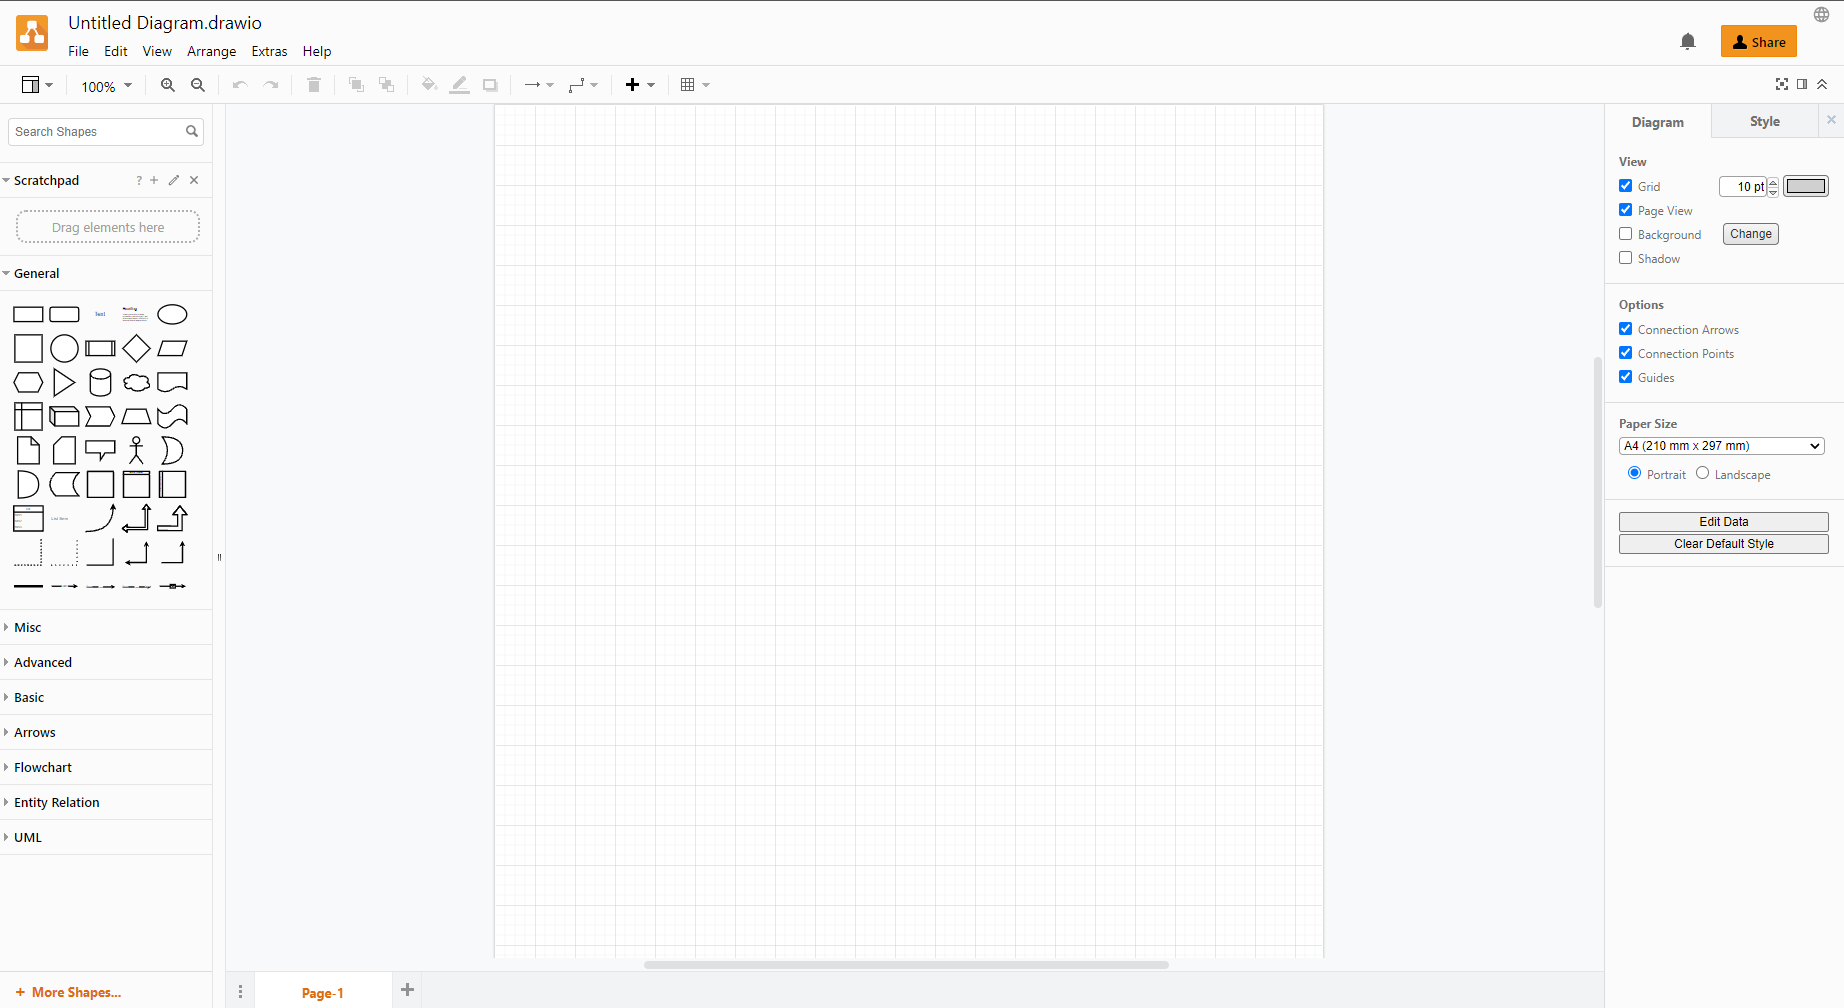
\includegraphics[width=\textwidth]{images/drawio.png}
	\caption{A draw.io kezelőfelülete \cite{drawio}}
\label{fig:drawio}
\end{figure}

\noindent
A kezelőfelület fejlécében az általános menüpontok szerepelnek. Az alkalmazás közepén van maga a felület, ahol az ábrák szerkeszthetők. Ezt fogja körbe a bal oldalról az ábrákkal kapcsolatos, még jobb oldalon a diagram beállításai, és előre definiált stílusok közül lehet választani. Az alapelemek csoportosítva vannak kinézetük alapján lenyitható menüpontokként. Az ábra kiválasztása után rögtön megjelenik a felület közepén, ezt követően lehet elhelyezni. Az ábrák szerkesztésénél több lehetőség áll fenn. Rendelkezik Undo-Redo funkciókkal, az elkészített diagram menthető különböző fájlformátumokban. Az előre definiált pár stíluson felül többféleképpen is meg lehet adni saját színeket is: RGB színválasztó, hexakódok, és gyakran használt színek egyaránt. Be lehet állítani az adott ábrára kitöltőszínt, betűszínt, vízszintes és függőleges igazítást, árnyékot, bemetszést, és még sok apróságot. Bármelyik ábrára helyezhető szöveg, ennek a stílusa igazodik hozzá. Az objektumok bárhol összekapcsolhatók, de megjelennek ajánlott pontok is: 0, 25, 50, 75 és 100\%-on. A rétegek nem jelennek meg külön oldalon, az ábrák sorrendje számít, hogy melyik jelenik meg felül. A kijelölés téglalap alapú, a kijelölt elemeket lehet másolni, törölni, szerkeszteni. Az ábrák csak rácspontokhoz igazíthatók.


\SubSection{TikZiT}
\begin{figure}[!h]
	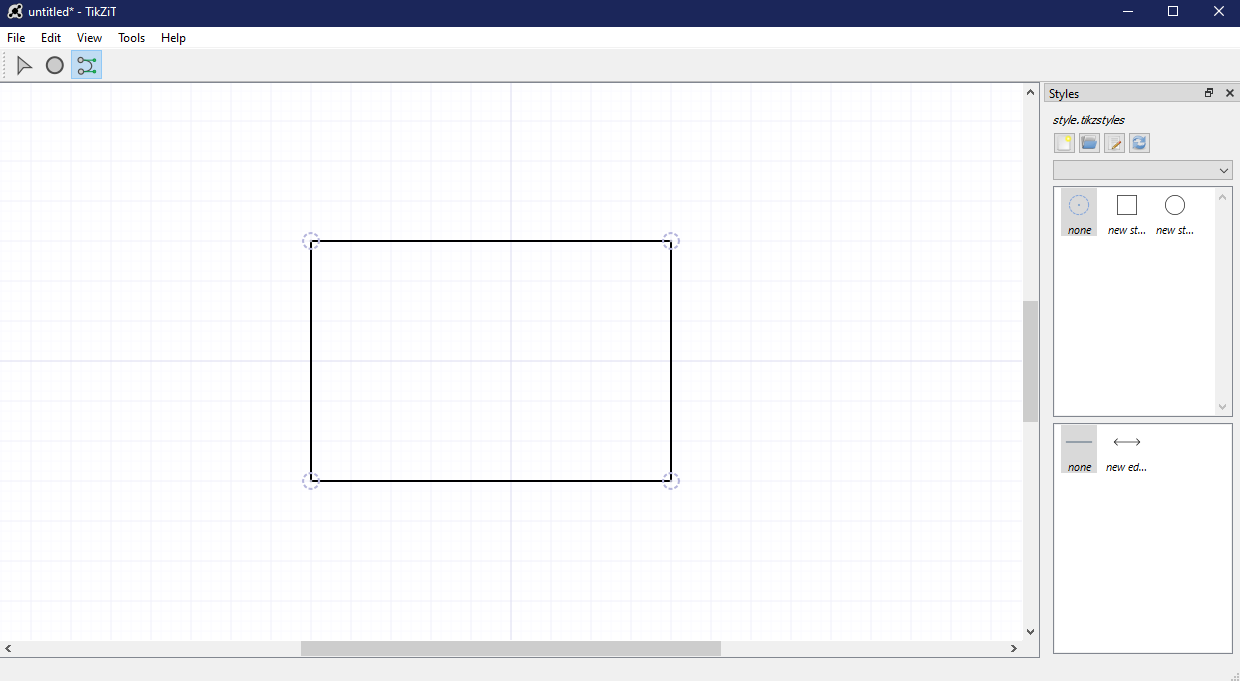
\includegraphics[width=\textwidth]{images/tikzit.png}
	\caption{A TikZiT kezelőfelülete \cite{tikzit}}
	\label{fig:tikzit}
\end{figure}

\noindent
A TikZiT inkább gráfok rajzolására használható, a vezérlő elemek az alkalmazás fejlécében helyezkednek el. A grafikus alapelemek szintén itt találhatóak, számuk nem kiemelkedő: a kijelölésen kívül van egy gráf csomópont lerakásához és egy gráf éleinek berajzolásához egy gomb. Mind a csomópont, mind a gráf stílusa módosítható, fájlként menthető, és betölthető, a programon belül és kívül is szerkeszthetők. Három lehetőség van: alak, szín, kitöltés. A szín és kitöltés kiválasztása történhet előre definiált alapszínekből, de lehetőség van RGB színskálából kiválasztásra vagy hexakód megadására is. Szöveg a gráf csomópontjainak adható. A csomópontokat összekötő élek a két pont helyzetétől függenek, csak az él hajlítására van lehetőség. A csomópontok rétegződését a lerakás sorrendje határozza meg, utólag csak kijelölés után van lehetőség előre vagy hátra küldeni az adott elemet. A kijelölés téglalap alakú, a kijelölt elemek másolhatók, törölhetők, stílusuk szerkeszthető.  A program rendelkezik Undo-Redo funkciókkal, a rajzolófelületen lehetőség van nagyításra és kicsinyítésre egyaránt. A kész ábrák mentése fájlba történik, automatikus mentés nincs, ezek betölthetők későbbi szerkesztésre is. 

\SubSection{TikzEdt}
\begin{figure}[!h]
	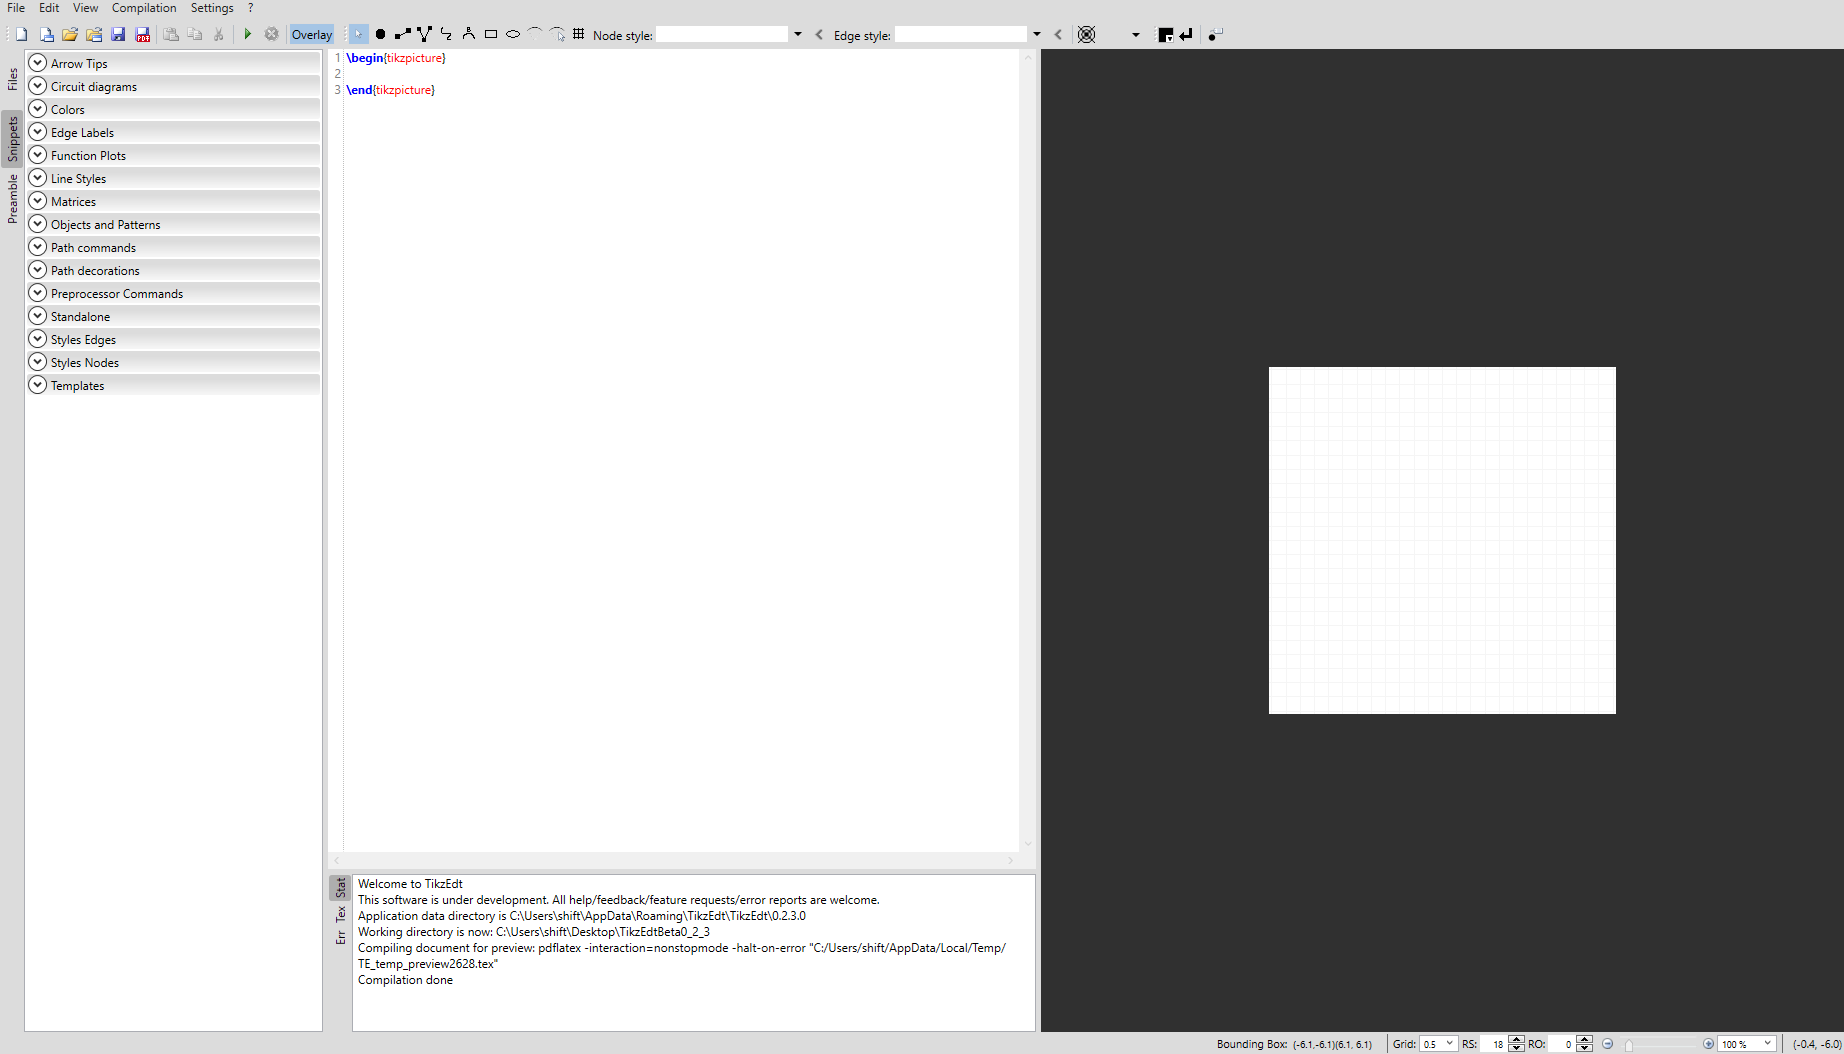
\includegraphics[width=\textwidth]{images/tikzedt.png}
	\caption{A TikzEdt kezelőfelülete \cite{tikzedt}}
\label{fig:tikzedt}
\end{figure}

\noindent
A TikzEdt esetében három hasábra osztható a felület: elsőben az előre definiált \LaTeX\ kódrészletek, másodikban a LaTeX kódszerkesztő, és végül a harmadikban a lefordított kód előnézete jelenik meg. Az alapelemek a felső sávban jelennek meg: főleg gráfokkal és egyszerűbb elemeket tartalmaz. Az elemek, gráfok, egyenletek, szövegek stílusa és színei csak kód szinten szerkeszthető, de vannak választható opciók. A rétegződés a lerakás sorrendjében van, utólag módosításra nincs lehetőség. Az elemek automatikusan rácspontokhoz igazodnak. A kijelölés téglalap alakú, a kijelölt elemek csak törölhetők.  A program rendelkezik Undo-Redo funkciókkal, a rajzolófelületen lehetőség van nagyításra és kicsinyítésre egyaránt. A kész ábrák mentése fájlba történik, automatikus mentés nincs.

\SubSection{tikzcd-editor}
\begin{figure}[!h]
	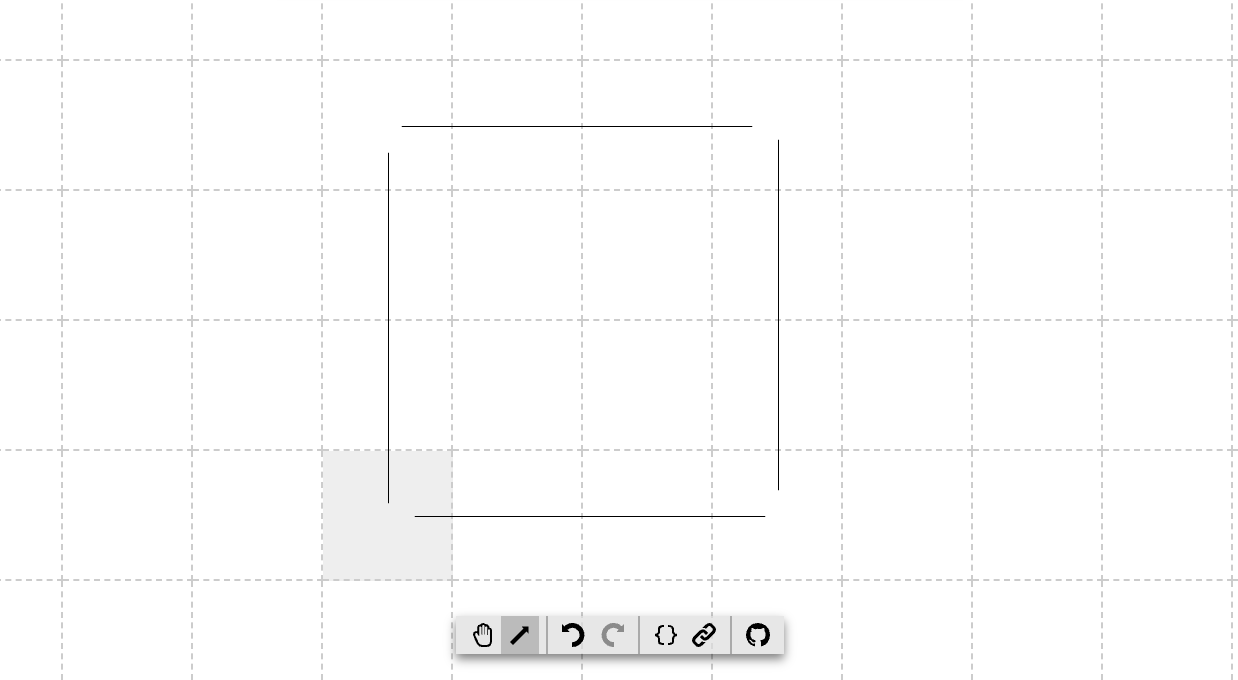
\includegraphics[width=\textwidth]{images/tikzcd.png}
	\caption{tikzcd-editor kezelőfelülete \cite{tikzcd}}
	\label{fig:tikzcd}
\end{figure}

\noindent
A tikzcd-editor klasszikus felülettel nem rendelkezik, csak egy négyzet alapú rendszer fogad megnyitáskor. A rácsok közepére igazítva lehet nyilakat rajzolni, és szövegeket írni, de utólag van lehetőség a fel-le mozgatásra. A stílusok nem testreszabhatók, csak pár alap stílusból lehet választani, mint a szaggatott vagy dupla vonal, módosítható a nyíl eleje, illetve vége. Az elemek színei nem módosíthatók, csak az alap fekete érhető el. A rétegződés a lerakás sorrendjében van. Kijelölés csak egyesével működik, nincs lehetőség téglalap vagy esetleg lasszó alapú kijelölésre. A program rendelkezik Undo-Redo funkciókkal, de mentésre nincs lehetőség, csak a \LaTeX\ kód kimásolására, és az ábrához tartozó link utólagos betöltésére.


\begin{table}[]
	\centering
	\begin{tabular}{|l|c|c|c|c|}
		\hline
		& draw.io & tikzit & tikzedt& tikzcd\\ \hline
		
		Elrendezés  & \multicolumn{3}{c|}{hasáb felépítés} & alul\\ \hline
		
		\begin{tabular}[c]{@{}l@{}}Property-k \\ szerkesztése\end{tabular}& \multicolumn{2}{c|}{előre definiált stílusok}& \begin{tabular}[c]{@{}c@{}}csak kód \\ szinten\end{tabular}& \begin{tabular}[c]{@{}c@{}}kijelölés \\ után\end{tabular} \\ \hline
		
		\begin{tabular}[c]{@{}l@{}}Színek megadási \\ módjai\end{tabular}& \multicolumn{2}{c|}{\begin{tabular}[c]{@{}c@{}}előre definiált színek, \\ RGB, és HEX  megadás\end{tabular}} & \begin{tabular}[c]{@{}c@{}}csak kód \\ szinten\end{tabular}& nem \\ \hline
		
		\begin{tabular}[c]{@{}l@{}}Alapelemek \\ megjelenítése\end{tabular}& \begin{tabular}[c]{@{}c@{}}mátrix alapú, \\ csoportosítva\end{tabular} & sorban & \begin{tabular}[c]{@{}c@{}}lenyíló listás \\ rendezés\end{tabular} & sorban \\ \hline
		
		\begin{tabular}[c]{@{}l@{}}Szövegek \\ szerkesztése\end{tabular}& igen & \multicolumn{2}{c|}{csak csomópontokon} &  \begin{tabular}[c]{@{}c@{}}rácsok \\ közepén\end{tabular} \\ \hline
		
		\begin{tabular}[c]{@{}l@{}}Objektumok\\ összekapcsolási\\ módjai\end{tabular} & bárhol & \multicolumn{2}{c|}{középen} & nem \\ \hline
		
		Rétegek kezelése & \multicolumn{4}{c|}{rajzolási sorrend} \\ \hline
		
		Kijelölés & téglalap alapú & \multicolumn{3}{c|}{kattintás alapú} \\ \hline
		
		Másolás & \multicolumn{2}{c|}{igen} & \begin{tabular}[c]{@{}c@{}}csak kód \\ szinten\end{tabular} & nem \\ \hline
		
		\begin{tabular}[c]{@{}l@{}}Undo-redo \\ funkciók\end{tabular} & \multicolumn{4}{c|}{igen} \\ \hline
		
		\begin{tabular}[c]{@{}l@{}}Automatikus \\ mentés\end{tabular} & igen & \multicolumn{3}{c|}{nem} \\ \hline
		
		Zoom-olás & \multicolumn{3}{c|}{igen} & nem \\ \hline
		
		\begin{tabular}[c]{@{}l@{}}Objektumok\\ automatikus \\ igazítása\end{tabular} & igen & \multicolumn{2}{c|}{nem} & igen \\ \hline
	\end{tabular}
\end{table}
\Chapter{Követelmények a saját szerkesztővel szemben}

% Kb. 8 oldal

Egy weboldal tartalmának felhasználói megértése gyakran attól függ, hogy a felhasználó hogyan érti meg a weboldal működését. Ez a felhasználói élménytervezés része. A felhasználói élmény az elrendezéssel, az egyértelmű utasításokkal és a címkézéssel függ össze egy weboldalon. Az, hogy a felhasználó mennyire érti meg, hogyan tud interakcióba lépni egy webhelyen, szintén függhet a webhely interaktív kialakításától. Ha a felhasználó érzékeli a weboldal hasznosságát, nagyobb valószínűséggel fogja azt továbbra is használni. Azok a felhasználók, akik gyakorlottak és jártasak a webhelyek használatában, ennek ellenére hasznosnak találhatnak egy markánsabb, de kevésbé intuitív vagy kevésbé felhasználóbarát webhelyfelületet. A kevésbé tapasztalt felhasználók azonban kisebb valószínűséggel látják a kevésbé intuitív weboldal-felület előnyeit vagy hasznosságát. Ez a tendencia az univerzálisabb felhasználói élmény és a könnyebb hozzáférés irányába mutat, hogy a lehető legtöbb felhasználónak megfeleljen, függetlenül a felhasználói készségektől. A felhasználói élménytervezés és az interaktív tervezés nagy részét figyelembe veszik a felhasználói felület tervezésénél.

\Section{Tipikus elrendezések vizsgálata}

A felhasználói felület kialakításának egy részét befolyásolja az oldal elrendezésének minősége. Az elrendezés tervezésekor például figyelembe kell venni, hogy a webhely oldalelrendezésének a különböző oldalakon konzisztensnek kell-e maradnia. Az oldal pixelszélessége szintén létfontosságúnak tekinthető az objektumok igazításához az elrendezés tervezésében. A legnépszerűbb fix szélességű weboldalak általában ugyanolyan beállított szélességgel rendelkeznek, hogy megfeleljenek az aktuálisan legnépszerűbb böngészőablaknak, az aktuálisan legnépszerűbb képernyőfelbontás mellett, az aktuálisan legnépszerűbb monitorméreten.

Az elkészült webes alkalmazás elrendezés szempontjából átláthatónak kell lennie, ehhez a legegyszerűbb megvalósítás a hasáb alapú elrendezés: két, esetleg három hasáb. Egyikben az alkalmazás menüje, másik hasábban pedig maga a szerkesztő foglal helyet, a harmadik hasábban a funkciókhoz tartozó ablak jelenjen meg. 

\begin{figure}[!h]
	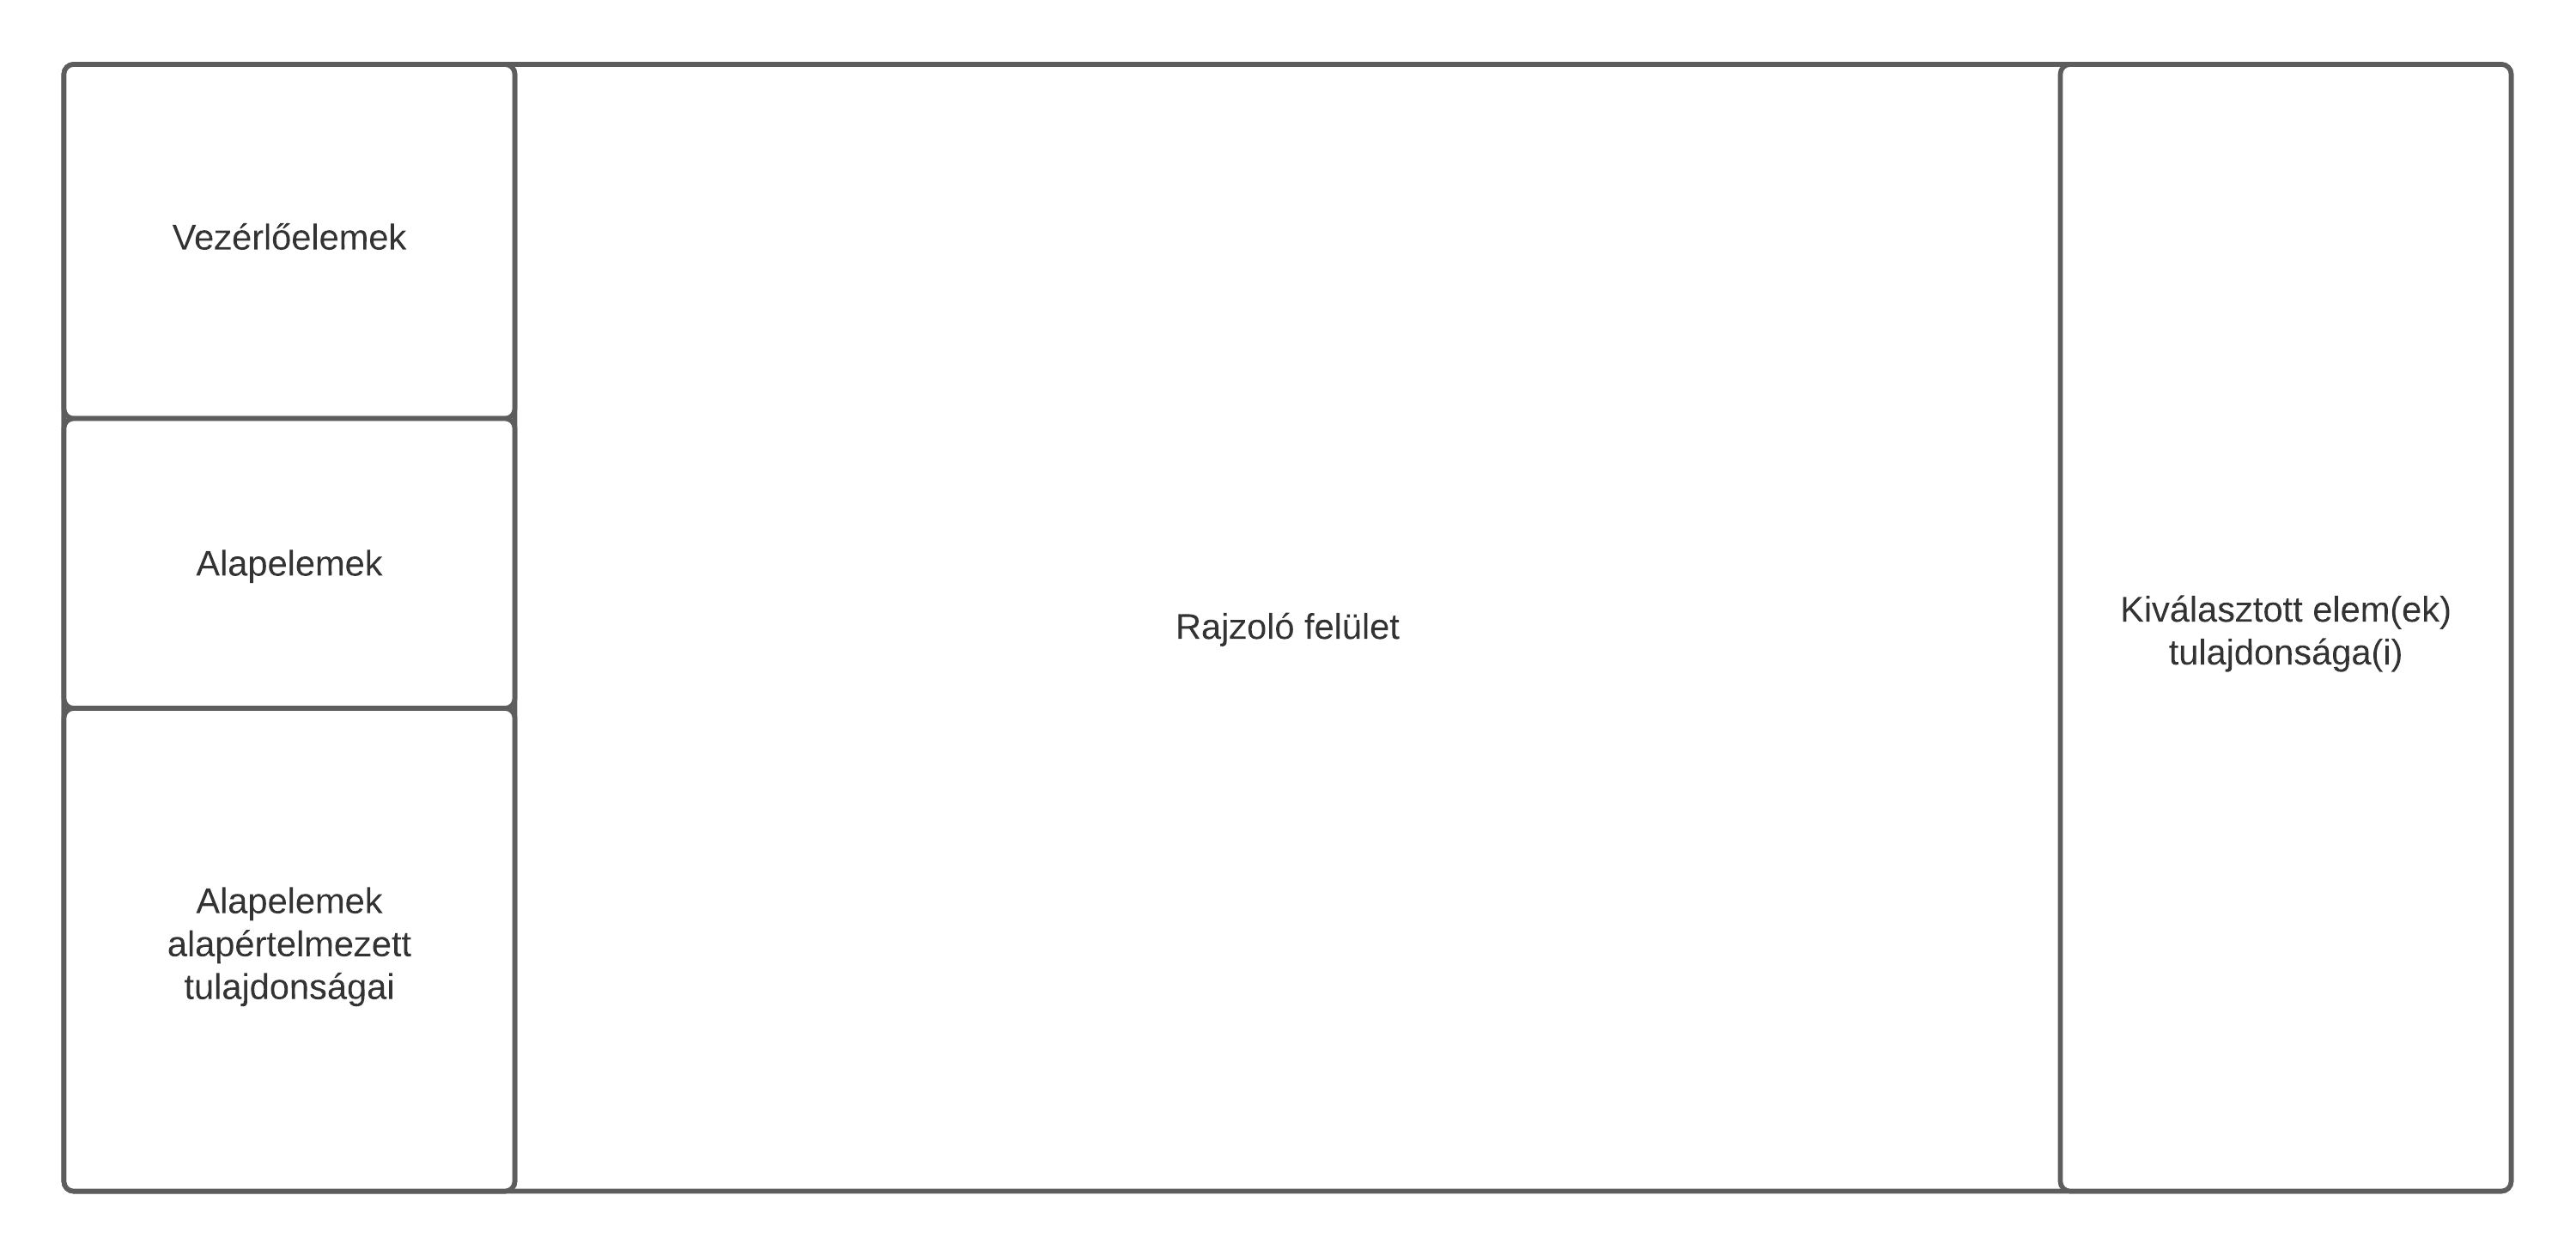
\includegraphics[width=\textwidth]{images/block.png}
	\caption{Az alkalmazás felépítése}
	\label{fig:block}
\end{figure}

Az alkalmazás legyen reszponzív akár a felület, akár a funkciók megjelenítése szempontjából. A reszponzív webdesign egy újabb megközelítés, amely a \textit{CSS3}-on és a \textit{CSS @media} szabály továbbfejlesztett használatán keresztül az oldal stíluslapján belül a készülékenkénti specifikáció mélyebb szintjén alapul. 

\Section{Alapelemek megjelenítése, és kiválasztása}

Az alapelemek megjelenése és kiválasztása egyaránt fontos a felhasználó megragadásában. Ha ezek átláthatók, és jól használhatók, akkor nagyobb célközönséghez juthat el az alkalmazásunk.

\SubSection{Alapelemek megjelenítése}

A funkciók a weboldal első hasábját foglalja magába, itt találhatók meg az alapelemek is a vezérlőelemeken és a kiválasztott elem tulajdonságainak kiválasztásán felül.  

Az alkotóelemek a kis hely miatt két oszlopban lelhetők fel, tehát az alkalmazás mátrix alapú elrendezést használ. Célszerű az elemeket csoportosítani olyan tulajdonságok alapján, amiben megegyeznek: például a vonal és a görbe jelenleg meg egymás mellett a mátrixban. 

\SubSection{Alapelemek kiválasztása}

A rajzolási mód kiválasztása után automatikusan ki legyen választva a mátrix első eleme, mint aktuális elem. Az alapelemek kiválasztása a mátrix alapú listában történik beavatkozással. A felhasználó egérrel kiválasztja a számára szükséges elemet. A kiválasztás után megjelenik az adott elemekhez tartozó tulajdonságok listája, amivel ezek módosíthatók is.

\Section{Tulajdonságok szerkesztési lehetőségei}

A tulajdonságok szerkesztése szintén fontos akár az új, akár a meglévő elemek tulajdonságait szeretnénk módosítani. A felhasználó nem feltétlenül csak fekete-fehér ábrákat szeretne szerkeszteni.

\SubSection{Új elemek esetében}

Új elemek esetében minden újonnan lerakott elemre érvényesüljön az itt megadott beállítás. Ez érinti az elemek színét, kitöltési színét, vonal vastagságát és mintázatát is. Az elemek kezdeti és végpontjai kattintásra kerülnek a vászonra. Ahol szükséges egyéb tulajdonság is, mint például körvonal esetében a kezdő és végszögek külön beírhatók legyenek.

\SubSection{Meglévő elemek esetében}

A már lent lévő elemek esetében kijelölés után minden tulajdonságnak szerkeszthetőnek kell lennie. Ehhez a szerkesztő jobb oldalán lévő hasáb ad majd helyet. A kijelölt elemek meglévő tulajdonságait be kell tölteni, és változtatás esetén az adott elem tulajdonságait ez alapján módosítani. Fontos, hogy csak a releváns tulajdonságok jelenjenek meg.

\Section{Színek megadási módjai}

A szerkesztőnek tudnia kell kezelni a színeket, és ezeknek kiválaszthatónak kell lenniük. Az \LaTeX\ által előre definiált színeket elérhetővé kell tenni a felhasználónak. 

A színek kiválasztásához célszerű valamilyen lenyíló menüt használni, ezzel megkönnyítve ezeknek az elérését. 

\begin{figure}[!h]
	\centering
	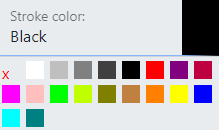
\includegraphics[]{images/colorpicker.png}
	\caption{Példa a színek kiválasztására}
	\label{fig:cp}
\end{figure}

Ebben az esetben megjelenítésre kerül a módosított tulajdonság, a kiválasztott szín, és a választható színek egyaránt. Az első elem a címek között jelöli azt, amikor nem kerül szín kiválasztásra: használható a körvonal eltüntetésére, vagy az ábra fehérrel történő kitöltés elkerülésére.

\Section{Objektumok automatikus igazítása}

Az alkalmazásnak tudnia kell kezelni a rácspontokat, és az ábrák egyes pontjait ezekhez kell igazítania. Az igazításnak meg kell történni ábra lerakásakor és már lent lévő elem kezdeti és végpontjai módosításakor. A Bézier-görbe esetében a kontrollpontok szintén paraméteresen módosíthatónak kell lenniük.

\Section{Objektumok összekapcsolási módjai}

A szerkeszthetőség érdekében lehetőséget kell adni a felhasználónak a már lent lévő objektumok összekapcsolására. Az összekapcsolás legegyszerűbb módja a pontok rácspontokhoz kapcsolása, és a kijelölés során lehetőséget adni több elem kijelölésére. Ebben az esetben a kijelölt pontok összekapcsolódnak, és mozgatásra együtt kerülnek kiszámolásra.

\Section{Szövegek szerkesztése}

Az alkalmazásnak kezelni kell a szöveget. A szövegeknek a vászonra lerakhatóknak és utólag szerkeszthetőeknek kell lenniük. 

A szövegekbe beletartoznak a \LaTeX\ matematikai módban írt kifejezései is, tehát például az $$ \int_{a}^{b} \qquad\qquad \bigcap_{a}^{b} \qquad\qquad \bigcup_{a}^{b} \qquad\qquad \sum_{a}^{b} \qquad\qquad \prod_{a}^{b}$$ kifejezéseknek meg kell tudnia jelenni.

\Section{Kijelölés}

Az alkalmazásnak lehetővé kell tenni az elemek kijelölését. A kijelöléshez egérbillentyűket kell használni. A kijelölés után az adott elemek tulajdonságait módosítani lehet, másolni, és törölni. 

 Téglalap alapú kijelölés esetén egyszerre több elem is kijelölhető, még a kattintás alapú kijelölés esetén egy kattintással csak egy elem jelölhető ki, esetleg funkciógombokkal (mint például a \textit{CTRL}, vagy az \textit{ALT} billentyű) van lehetőség több elemet kijelölni.

\Section{Másolás és beillesztés}

A "\textit{másolás és beillesztés}" kifejezés a szöveg vagy más adatok forrásból a célba történő másolásának népszerű, egyszerű módszerére utal. A módszer népszerűsége az egyszerűségéből ered, valamint abból, hogy a felhasználók vizuálisan - állandó tárolás nélkül - könnyen mozgathatják az adatokat a különböző alkalmazások között. Miután adatokat másoltunk a vágólapra, a vágólap tartalmát beilleszthetjük a céldokumentumba.

\SubSection{Másolás}

A kijelölt elemek másolása billentyű lenyomásra működjön, megszokott alapon a \textit{C} billentyűre vagy a \textit{CTRL + C} billentyűkombinációra. A kijelölt elemek tulajdonságai (pozíció, szín, kitöltési szín...) kerüljenek mentésre egyaránt. 

\SubSection{Beillesztés}

A másolt elemek beillesztése szintén billentyű lenyomásra működjön, megszokott alapon a \textit{V} billentyűre vagy a \textit{CTRL + V} billentyűkombinációra. 

A beillesztett elemek ne a másolt elemeken, hanem kicsit eltolva jelenleg meg az átláthatóság és könnyebb szerkeszthetőség érdekében.

\Section{Kicsinyítés és nagyítás}

Az oldal nagyításának két különböző módja van:

\begin{itemize}
	\item a szövegek átméretezése a betűméret növelésével vagy csökkentésével, a vízszintes görgetés elkerülése érdekében a képek méretének változatlanul hagyásával.
	\item valódi átméretezés, amely a képeket, egyéb multimédiás objektumokat és a nézetablakokat is átméretezi.
\end{itemize}

Az alkalmazásnak támogatnia kell a kicsinyítését és nagyítását, legalább a vásznon megjelenő alapelemek méretének nagyításával vagy csökkentésével. Ezt célszerű az egér görgőjére hivatkozva módosítani: ha felfelé görgetünk, akkor nagyítsuk a vásznak, ellenkező esetben kicsinyítjük.

\Section{Undo-redo funkciók}

Az elkészült alkalmazásnak biztosítani kell a visszavonás és az újra lerakás funkcióit. Sokszor fordul az elő, hogy a felhasználó véletlenül más elemet rajzol a vászonra, vagy esetleg más elem tulajdonságait módosítja, így a felhasználói élmény növelése céljából szükség van ezeknek a hibáknak a visszavonására.

\Section{Mentés, és automatikus mentés}

\SubSection{Mentés}

Mentés során a felhasználó megkapja a szerkesztett ábrát \LaTeX\-be visszailleszthető állapotba. Ez egyaránt jelenti a \LaTeX\ kódot, valamint egy opcionálisan letölthető \textit{.tex} formátumú fájlt, amely az \textit{input} paranccsal betölthető tetszőleges \LaTeX\ állományba.

A mentés során a felhasználó kap egy hivatkozási kódot is, amely a későbbi betöltéshez szükséges. Ez egy \textit{BASE64} kódolású szöveg lenne, amelynek az a jelentősége, hogy elfedje a háttérben lévő "adatbázist", amelyből a kimentéshez szükséges \textit{JSON} objektumot kapjuk.

\SubSection{Automatikus mentés}

Az automatikus mentés számos számítógépes alkalmazás és videojáték mentési funkciója, amely automatikusan elmenti a program vagy játék aktuális változásait vagy előrehaladását, így segít csökkenteni az adatvesztés kockázatát vagy hatását összeomlás, lefagyás vagy felhasználói hiba esetén. Az automatikus mentés jellemzően vagy előre meghatározott időközönként, vagy egy összetett szerkesztési feladat megkezdése előtt, közben és után történik. Hagyományosan olyan funkciónak tekintették, amely alkalmazás- vagy rendszerhiba (például összeomlás) esetén védi a dokumentumokat, és az automatikus mentéses biztonsági mentéseket gyakran törlik, amikor a felhasználó befejezi a munkáját. A megvalósítás a fájl, az alkalmazás és az operációs rendszer szintjén is kihívásokkal jár.

Ezek alapján az alkalmazásnak támogatnia kell az automatikus mentés funkciót. A legegyszerűbb megvalósítása ennek a fix időközönkénti állapotmentés. Web alkalmazás révén ehhez a megoldás a \textit{HTTP-süti}k használata.

A HTTP-sütik (vagy más néven böngészősütik vagy egyszerűen sütik) olyan kis adatblokkok, amelyeket egy webszerver hoz létre, miközben a felhasználó egy webhelyet böngészik, és amelyeket a  webböngésző helyez el a felhasználó számítógépén vagy más eszközén. A sütik a weboldal eléréséhez használt eszközön kerülnek elhelyezésre, és egy munkamenet során egynél több süti is elhelyezhető a felhasználó eszközén.






\Chapter{JavaScript implementáció}

\Section{A p5 függvénykönyvtár}

Az elkészült szerkesztő jelentős mértékben támaszkodik a \textit{p5.js} függvénykönyvtár adta lehetőségekre. A \textit{p5} oldalán az alábbi ismertető olvasható:

"A p5.js egy JavaScript könyvtár a kreatív kódoláshoz, amelynek középpontjában az áll, hogy a kódolást elérhetővé és befogadóvá tegye művészek, tervezők, oktatók, kezdők és bárki más számára! A p5.js ingyenes és nyílt forráskódú, mert hiszünk abban, hogy a szoftvereknek és a tanuláshoz szükséges eszközöknek mindenki számára elérhetőnek kell lenniük.

A vázlat metaforáját használva a p5.js teljes körű rajzolási funkcionalitással rendelkezik. Azonban nem korlátozódik a rajzvászonra. Az egész böngészőoldalt tekintheted vázlatodnak, beleértve a HTML5-objektumokat a szöveghez, a bevitelhez, a videóhoz, a webkamerához és a hanghoz\cite{p5js}."

\SubSection{Telepítés}

A p5 függvénykönyvtár telepítéséhez csak hozzá kell adni a fájlunkhoz:

\begin{lstlisting}[style=html]
<html>
	<head>
		<script src="../p5.min.js"></script>
		<script src="sketch.js"></script>
	</head>
	<body>
	</body>
</html>
\end{lstlisting}

\SubSection{Használat}

A p5.js függvényhívások a \textit{sketch.js}-ben kapnak helyet globális névtér használat esetében:

\begin{lstlisting}[style=es6]
function setup() {
	createCanvas(400, 400);
}

function draw() {
	background(220);
	ellipse(50, 50, 80, 80);
}
\end{lstlisting}

A \textit{setup} függvény a \textit{sketch.js} betöltésekor fut le, célszerű iderakni a p5 vászon létrehozását (\textit{createCanvas} függvényhívás, mely paraméterként várja a magasságot és a szélességet). A \textit{draw} függvény a futás során folyamatosan meghívódik.

A dolgozatban a \textit{p5.js} példányosított módban fut a modulok miatt.
\begin{lstlisting}[style=es6, morekeywords={P5}]
const sketch = s => {
	
	s.setup = () => {
		setup();
	}
	
	s.draw = () => {
		draw();
	}

...

}

const P5 = new p5(sketch);

export {
	P5
}
\end{lstlisting}

Ebben az esetben a \textit{P5} névtér alá kerül a vászon, és a modulokban importálni kell a névtér hivatkozását, valamint az eddig globális \textit{p5.js} függvényhívások is ezen névtér alá kerülnek. Ebben az esetben a fenti példa így kerül definiálása:

\begin{lstlisting}[style=es6, morekeywords={P5}]
import {P5} from "../sketch.js";

const setup = () => {
	P5.createCanvas(400, 400);
}

const draw = () => {
	P5.background(220);
	P5.ellipse(50, 50, 80, 80);
}
\end{lstlisting}

\Section{Az alkalmazás felépítése}

Az alkalmazás a \ref{fig:block}. ábrán lévő blokkdiagram alapján készült el. Az ábrán lévő elemek nem minden funkcióban jelennek meg. A következő fejezetekben az egyes funkciók képernyői láthatók. 

A fejezetben megjelenő képernyő mintaképeken a vászon ötszörös nagyításban van a jobb átláthatóság miatt.

\SubSection{Kezdőképernyő} 

Ez a képernyő jelenik meg az alkalmazás betöltésekor. A bal oldali menüben automatikusan ki van választva a vászon mozgatására alkalmas funkció.

Az egér bal gombjával tudjuk pozicionálni míg görgővel kicsinyíteni vagy nagyítani a vásznat. Az egér középső gombját lenyomva pedig az alapértelmezett pozícióra és nagyításra visszaáll a vászon.

\begin{figure}[!h]
	\label{fig:canvas}
	\centering
	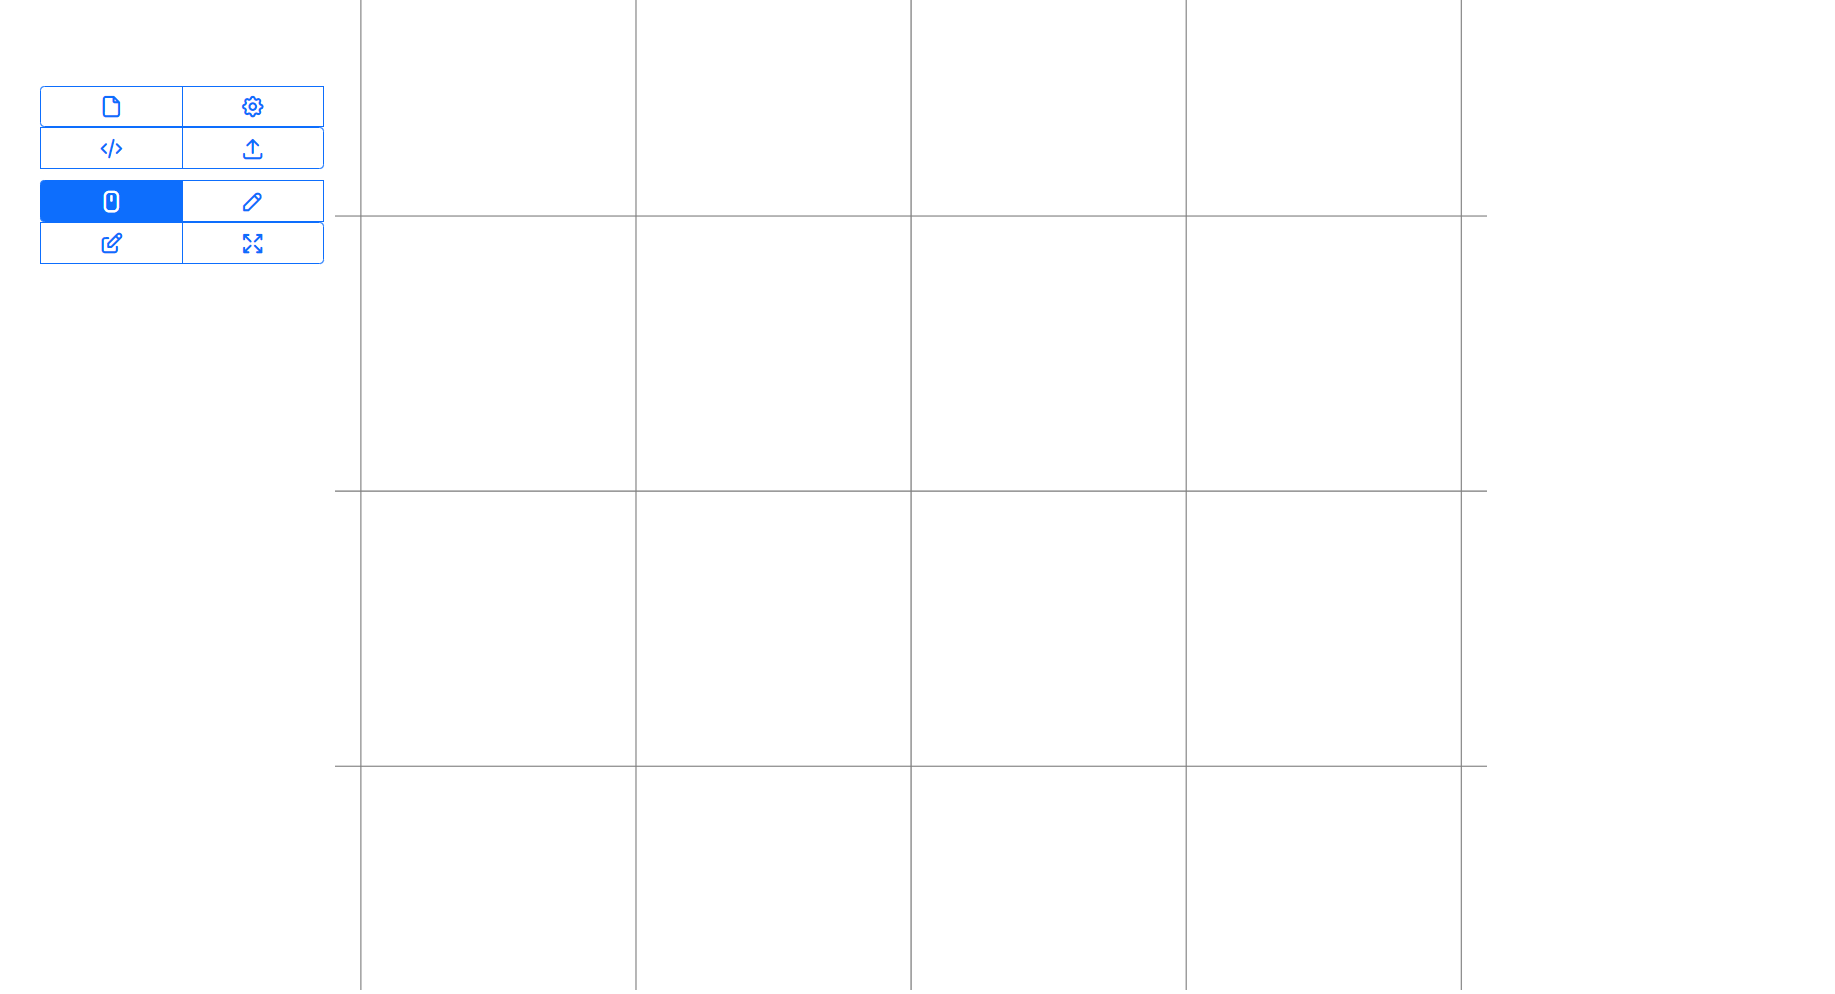
\includegraphics[width=\textwidth]{images/editor_canvas.png}
	\caption{Az elkészült alkalmazás kezdőképernyője}
\end{figure}

Az alkalmazás bármely menüpont alatt támogatja a visszavonás műveleteit: az adott művelet visszavonható a \textit{CTRL + Z} billentyűkombinációval, míg a \textit{CTRL + Y} kombináció lehetőséget biztosít a visszavont művelet megismétlésére. 

\SubSubSection{Vezérlőgombok}

A bal oldalt megjelenő gombok közül a felső mátrix biztosítja az új dokumentum létrehozását, a beállításokat, a meglévő ábra mentését, és visszatöltését.

Az első ikonra 
(
\includegraphics[height=\fontcharht\font`\B]{images/new.png})
kattintva új dokumentumot hozhatunk létre. Ekkor a már meglévő ábra eltűnik, visszatöltésre nincs lehetőség.

\begin{figure}[!h]
	\label{fig:new}
	\centering
	
\includegraphics[width=0.75\textwidth]{images/new_modal.png}
	\caption{Új dokumentum létrehozásakor megjelenő figyelmeztető üzenet}
\end{figure}

A fogaskerék ikonnal 
(
\includegraphics[height=\fontcharht\font`\B]{images/settings.png})
megnyithatjuk a beállításokat, itt van lehetőség az alapértelmezetten bekapcsolt rácsponthoz illeszkedést kikapcsolni, és az előnézetet bekapcsolni.

A következő két ikon felelős a már kész ábra kimentésére 
(
\includegraphics[height=\fontcharht\font`\B]{images/save.png}),
valamint a letöltött ábra visszamásolására
(
\includegraphics[height=\fontcharht\font`\B]{images/load.png}).

Az ábra kimentésekor egy felugró ablak fogad. Ekkor mentésre kerül a jelenlegi vászon állapota is süti formájában. A hivatkozási kód és a \textit{Tikz} kód kimásolható a mezőből gombnyomásra is, valamint egybefűzve le is tölthetők. Ebben az esetben a letöltött \textit{.tex} fájlban egymás alatt jelenik meg a hivatkozási kód, a \textit{TikZ} ábra kódja, valamint a letöltött állomány létrehozásának időpontja. Ezek a \textit{.tex} fájlok módosítás nélkül importálhatók az \lstinline[style=latex]{\input} paranccsal a meglévő dokumentumokba. 

\begin{figure}[!h]
	\label{fig:load}
	\centering
	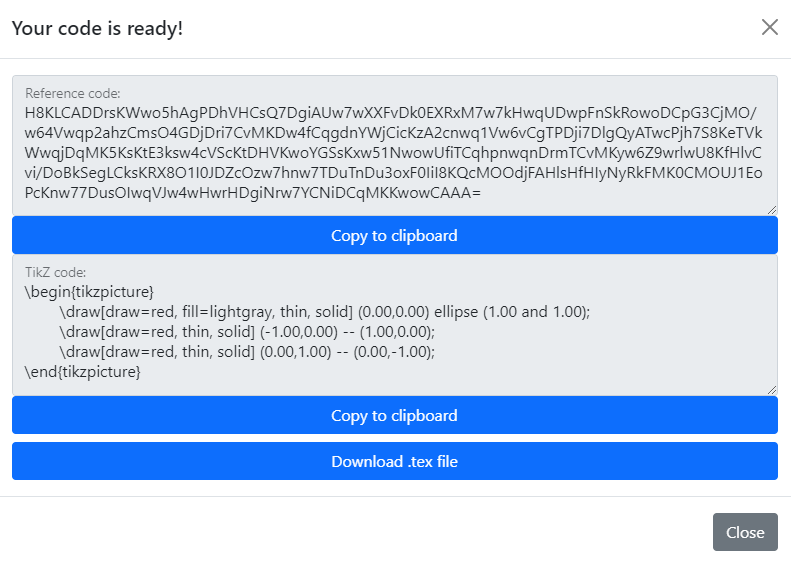
\includegraphics[width=0.75\textwidth]{images/save_modal.png}
	\caption{Az ábra mentésekor megjelenő ablak}
\end{figure}

Az ábra betöltésekor a már meglévő hivatkozási kód bemásolása után az alkalmazás betölti a kódhoz tartozó ábrát és kezdhetjük is a már meglévő ábra szerkesztését és kibővítését.

\begin{figure}[!h]
	\label{fig:save}
	\centering
	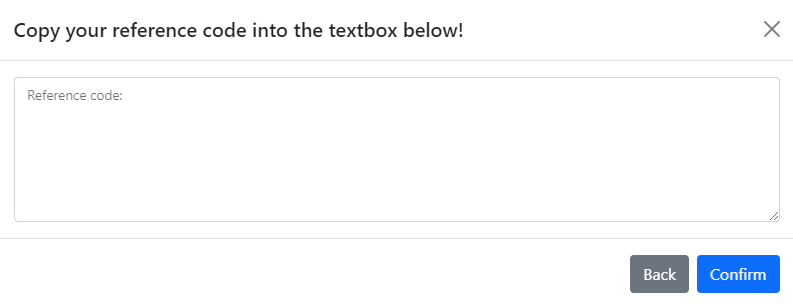
\includegraphics[width=0.75\textwidth]{images/load_modal.png}
	\caption{Az ábra betöltésekor megjelenő ablak}
\end{figure}

\SubSection{Rajzolás}

A rajzolás mód kiválasztásával megjelennek a vezérlőelemek alatt az alapelemek mátrix alapú felsorolásban és a kijelölt elemhez tartozó tulajdonságok.

A megfelelő tulajdonságok beállítása után a rajzolás az egérrel történik. A pont, szöveg és matematikai kifejezések kirajzolása kattintásra történnek, míg a maradék alapelem "drag and drop" (\textit{fogd és vidd}) megoldással kerül kirajzolásra, vagyis a kezdőpont a kattintás helye, és a végpont az egér gombjának felengedésének a pozíciója lesz.

\begin{figure}[!h]
	\label{fig:draw}
	\centering
	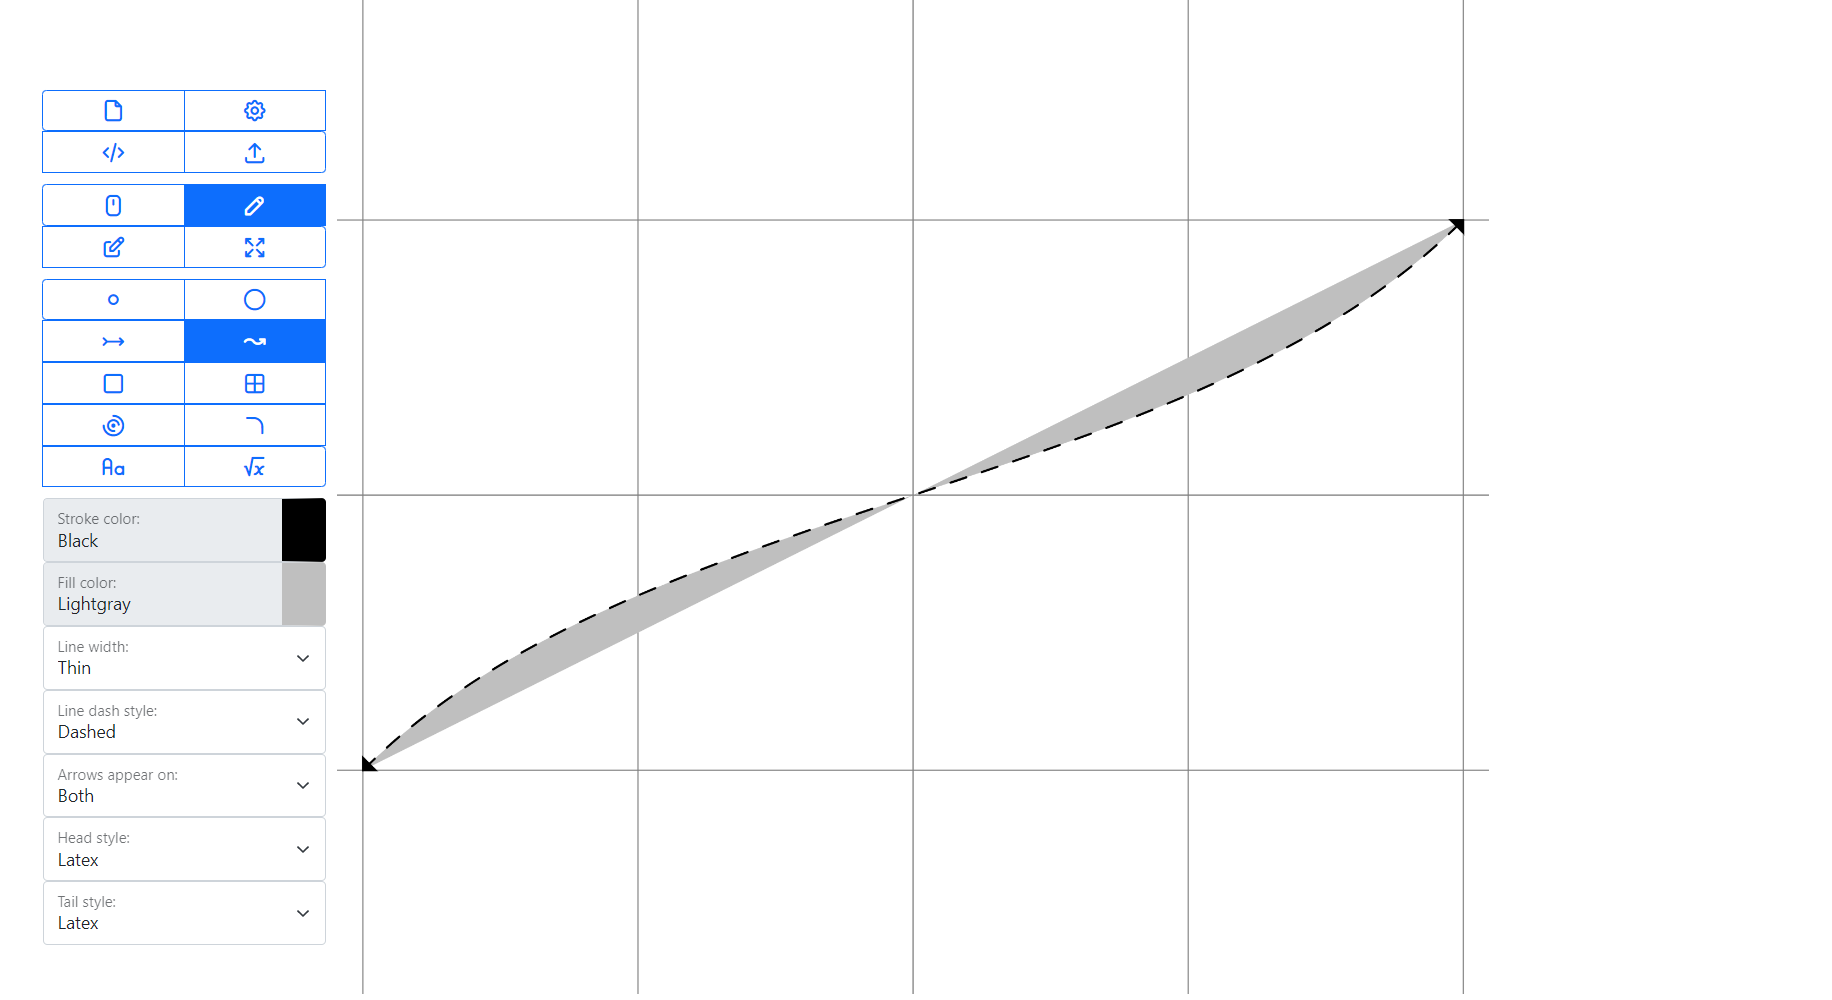
\includegraphics[width=\textwidth]{images/editor_draw.png}
	\caption{A rajzolás funkciói rajzolt elemmel a vásznon}
\end{figure}

Amennyiben az előnézet be van kapcsolva a beállításokban, úgy megjelenik az egér helyén egy körvonal, amely jelzi a rajzolandó elem kezdőpontját, valamint a szöveg és a matematikai kifejezések esetében a teljes tartalom megjelenik a beállított tulajdonságok szerint.


\SubSection{Szerkesztés}

A szerkesztés funkcióban lehetőség van a már lent lévő elemek kiválasztására. A kijelölés téglalap alakú, és a kezdő- és végpont szintén "drag and drop" módszerrel kerül megállapításra. A kijelölés közben egy világosszürke téglalap jelzi az aktuális kijelölt területet, így látszódik mely alapelemek esnek bele.

\begin{figure}[!h]
	\label{fig:edit}
	\centering
	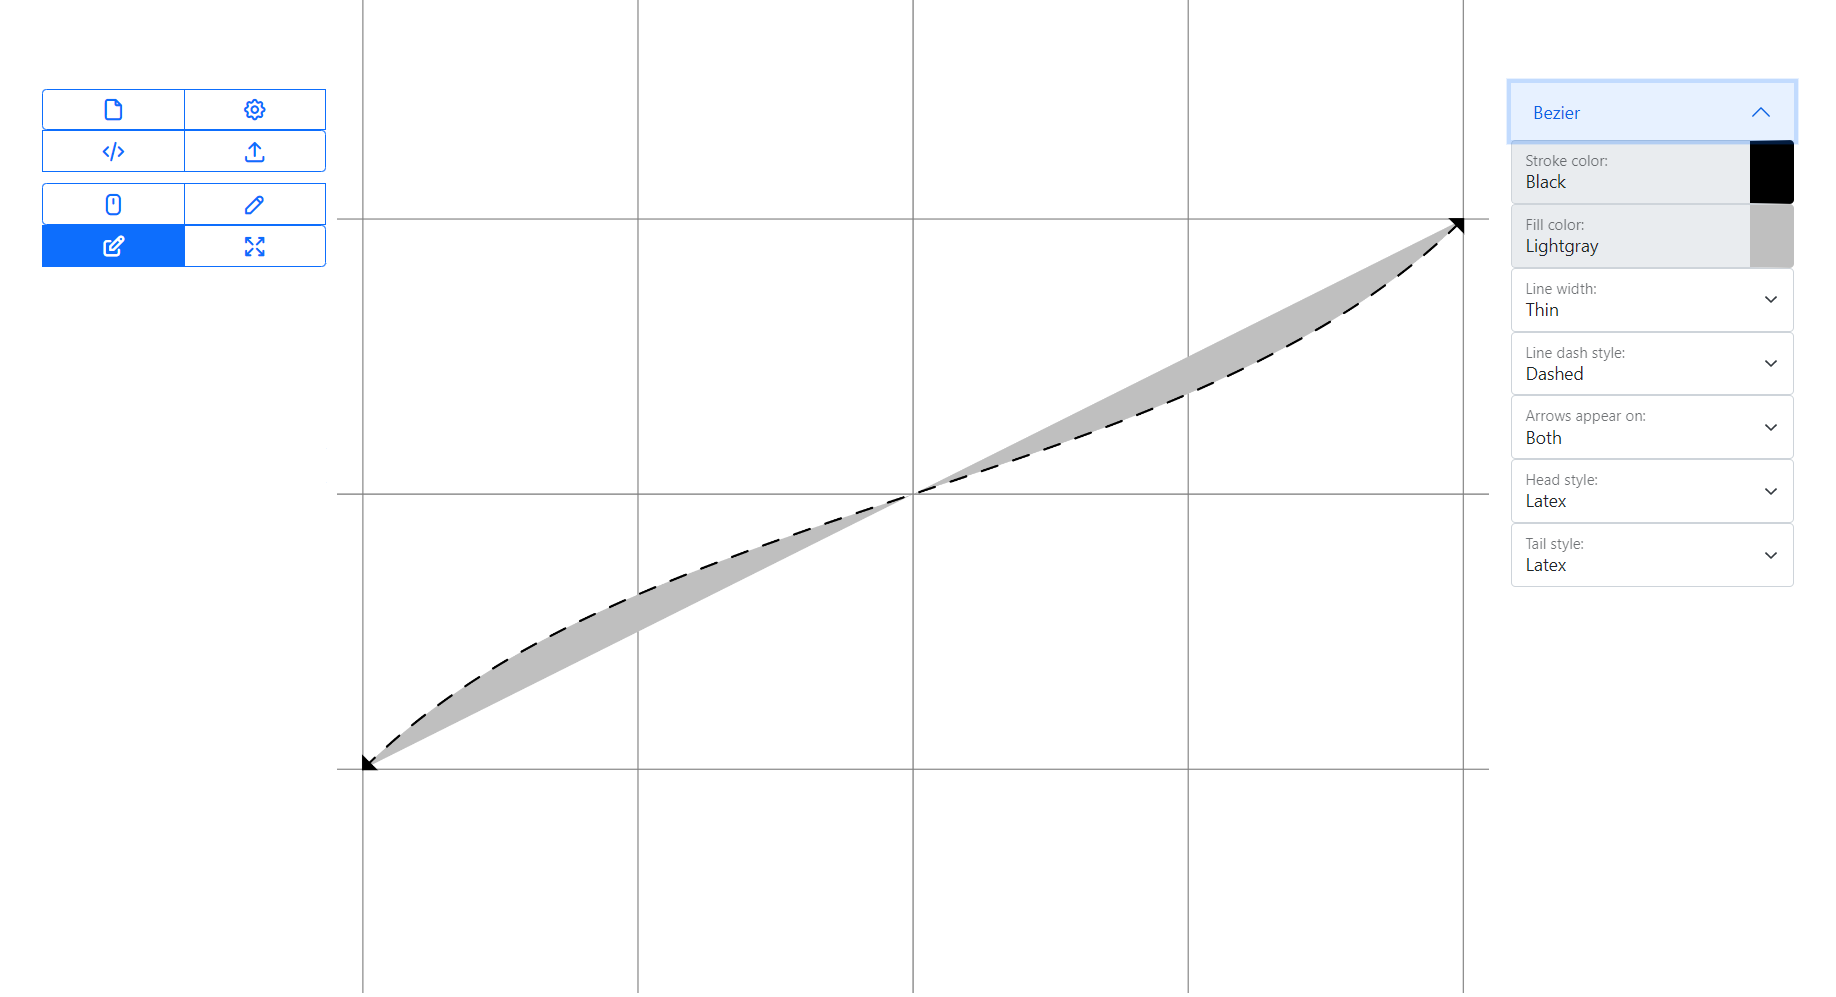
\includegraphics[width=\textwidth]{images/editor_edit.png}
	\caption{A szerkesztés képernyő kiválasztott elem után}
\end{figure}

A kijelölés véglegesítése után a rajzoló felület jobb oldalán megjelennek a kijelölt területbe beleeső alapelemek. Itt lehetőség van egyenként szerkeszteni a már lent lévő elemek tulajdonságait. A jelenlegi tulajdonságok automatikusan betöltődnek, módosításkor a vásznon automatikusan megjelenik, nincs szükség a módosítás mentésére.

Kijelölés után lehetőségünk van a másolásra, beillesztésre és törlésre egyaránt, ezek mindegyike billentyű lenyomásra működnek. A másolás a  \textit{CTRL + C}, a beillesztés a \textit{CTRL + V}, még a törlés a \textit{CTRL + X} billentyűkombinációval, és a \textit{DELETE} billentyűvel egyaránt működik.

\SubSection{Mozgatás}

A mozgatás funkcióban lehet a már lent lévő ábrák pontjait kijelölés után mozgatni. A mozgatandó elem kijelölése kattintásra történik, \textit{CTRL} billentyű lenyomása közben van lehetőség több pont kijelölésére. A mozgatás szintén "drag and drop" megoldással működik.

\begin{figure}[!h]
	\label{fig:move}
	\centering
	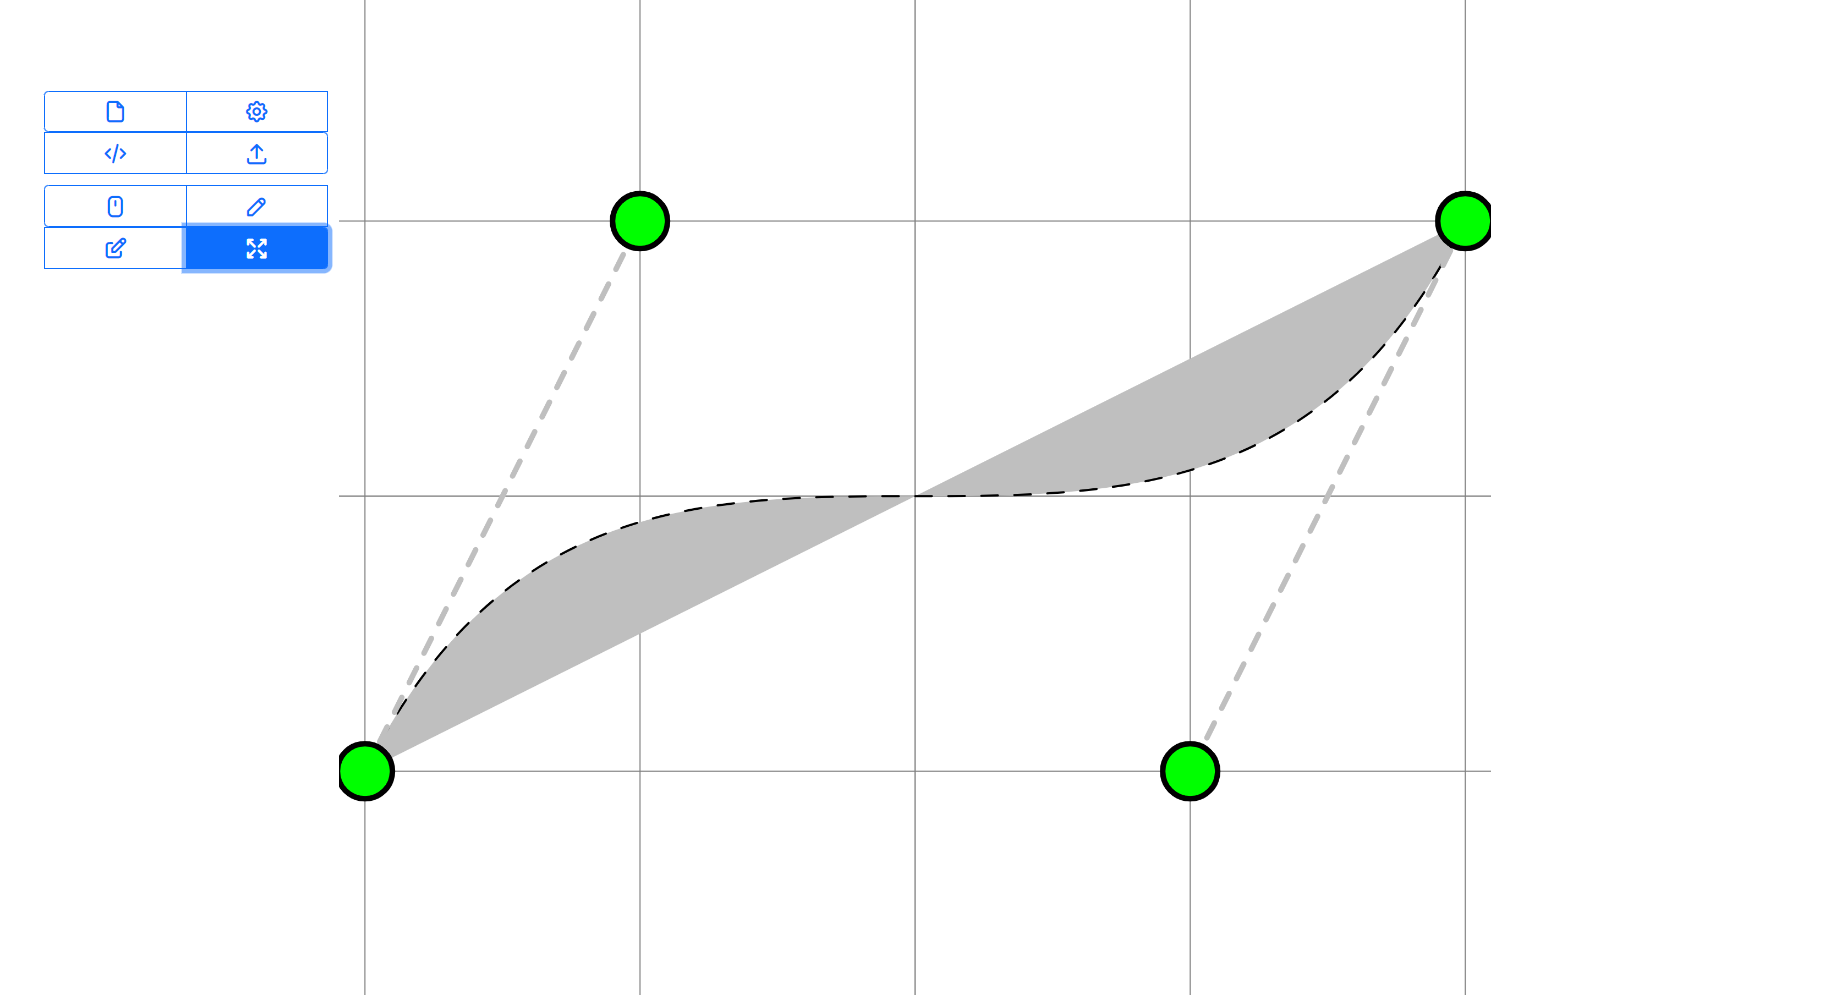
\includegraphics[width=\textwidth]{images/editor_move.png}
	\caption{A mozgatásra alkalmas pontok megjelenítése a vásznon}
\end{figure}

\Section{Definiált osztályok bemutatása}

\begin{figure}[!h]
	\centering
	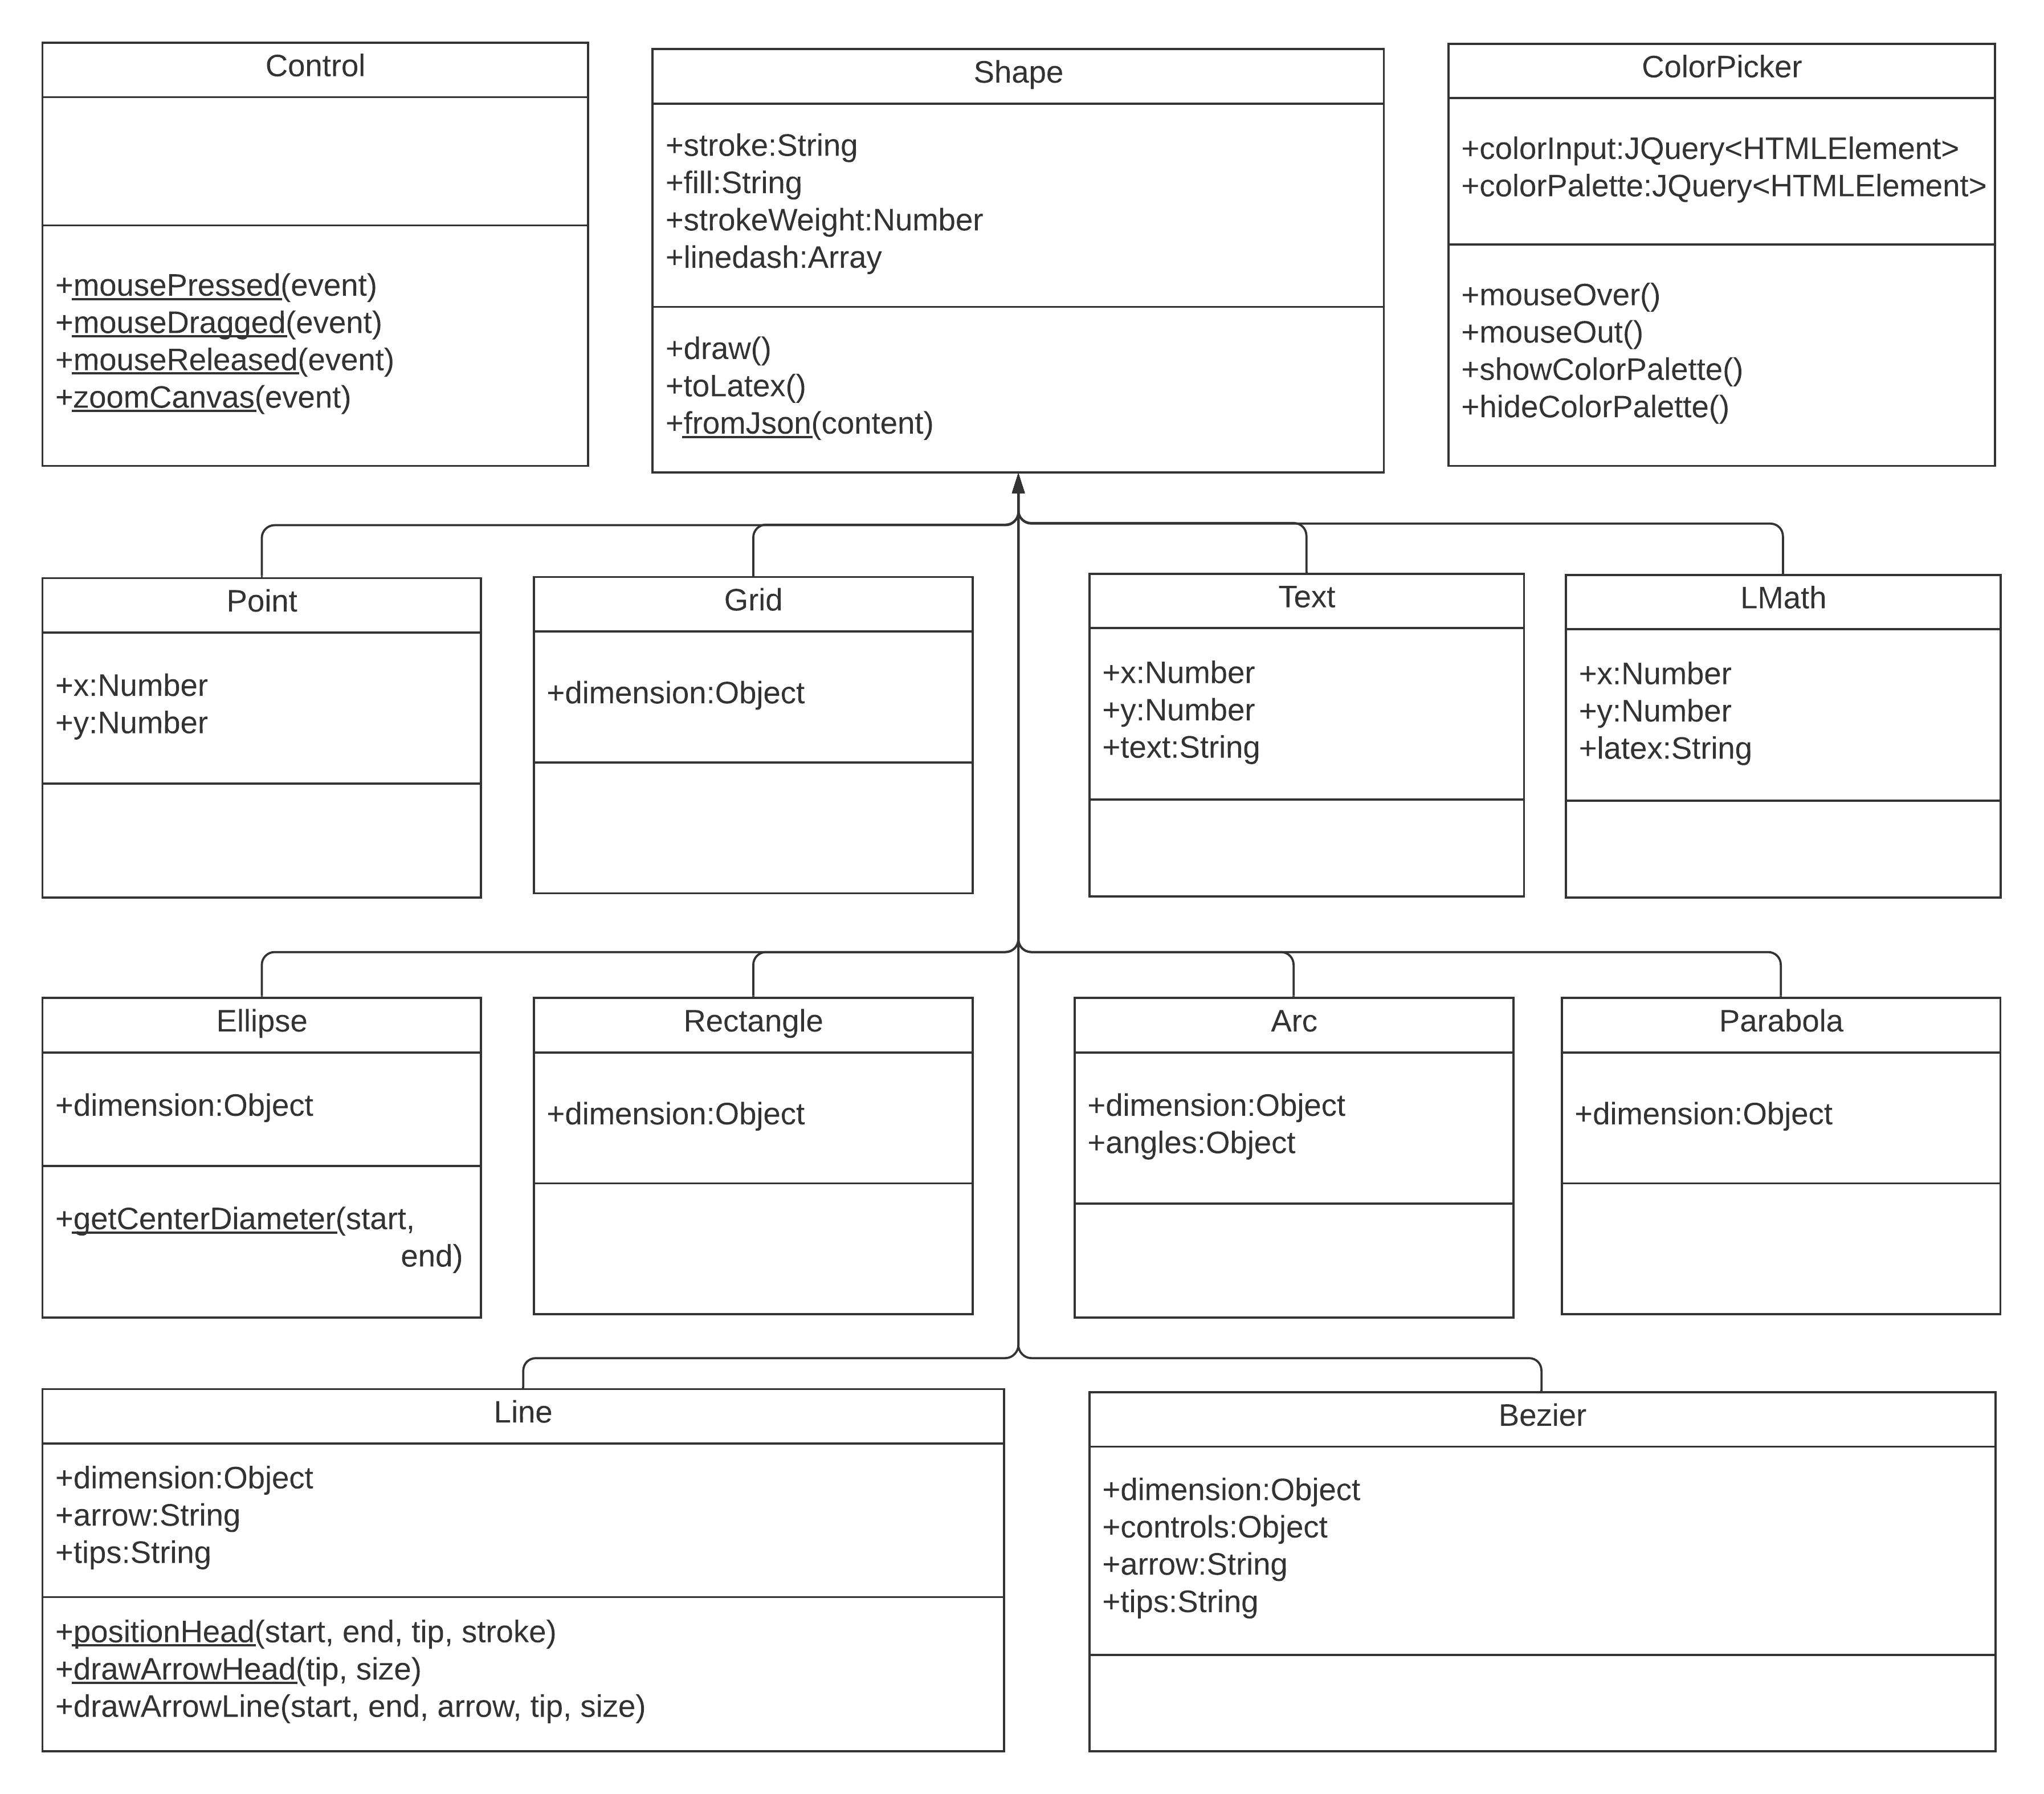
\includegraphics[width=\textwidth]{images/uml.png}
	\caption{Az osztályok UML diagrammja}
	\label{fig:uml}
\end{figure}

\SubSection{Alapelemek osztályai}

Ebbe a részbe kerülnek a menüben kiválasztható alapelemek osztályai, valamint az aktuális elem esetében a  \textit{p5.js} és \textit{TikZ} közötti különbségek és megoldásuk. 

\SubSubSection{Shape osztály}

A \textit{Shape} osztály minden alapelem szülője, itt kerül beállításra a majdnem az összes elemnél előforduló szín, betűszín, vonal vastagság és mintázat. A \textit{draw} metódus beállítja a megadott tulajdonságokat a rajzolás előtt. A \textit{toLatex} és a \textit{fromJson} metódusok még itt üresek, értékeket a származtatott osztályokban kapnak.

\SubSubSection{Point osztály}

A \textit{Point} osztály egy pont tulajdonságait tárolja. Példányosítás során meg kell adni a pont két koordinátáját, és a tulajdonságokat tömb formájában. A jobb láthatóság érdekében \textit{p5.js} és \textit{TikZ} esetében egy kis méretű kör kerül kirajzolásra. 

\SubSubSection{Ellipse osztály}

Az \textit{Ellipse} osztály ellipszis rajzolását teszi lehetővé. A példányosításhoz meg kell adni két koordinátapárt (egy x és egy y koordinátát), valamint a tulajdonságokat. A \textit{p5.js} és a \textit{TikZ} is ugyanúgy támogatja az ellipszis rajzolását: meg kell adni a középpontot és a sugár méretét, így szükséges egy metódus, ami ezt kiszámolja. A \textit{getCenterDiameter} metódus ezt teszi lehetővé:

\begin{lstlisting}[style=es6]
static getCenterDiameter(start, end) {
	let center = {
		x: start.x + (end.x - start.x) / 2,
		y: start.y + (end.y - start.y) / 2
	};

	let diameter = {
		x: end.x - start.x,
		y: end.y - start.y
	};
	return {center, diameter}
}
\end{lstlisting}

\SubSubSection{Line osztály}

A \textit{Line} osztályban vannak definiálva a vonal rajzolásához szükséges metódusok. A példányosításhoz meg kell adni két koordinátapárt (egy x és egy y koordinátát), valamint a tulajdonságokat. A nyilak rajzolását is ez az osztály végzi, ugyanis tulajdonságként megkapja, hogy hol és milyen típusú nyíl kirajzolása szükséges. 

A \textit{p5.js} megvalósítás kicsit komplikáltabb, mint a \textit{Tikz} megoldás. A \textit{p5.js} esetében a \textit{positionHead} metódus a kiválasztott végpontra lép, a \textit{drawArrowHead} metódus pedig az aktuális pontra kirajzolja a kiválasztott nyílhegyet. A \textit{drawArrowLine} metódus csak egyszerűen összeköti a két végpontot a nyílhegy függvényében.

A \textit{TikZ} esetében pedig csak a \textit{draw} paramétereként meg kell adni a nyílhegyet.

\SubSubSection{Bezier osztály}

A \textit{Bezier} osztály egy harmadfokú Bézier-görbe kirajzolását teszi lehetővé. A példányosításhoz meg kell adni két koordinátapárt (egy x és egy y koordinátát), valamint a tulajdonságokat. A program automatikusan számol lerakáskor két kontrollpontot a harmadolópontok helyére, mely utólag természetesen módosítható. A vonalaknál látott nyílhegyek itt is elérhetők.

A \textit{p5.js} és a \textit{TikZ} megadás rendre megegyezik: először meg kell adni a kezdőpontot, majd a két kontrollpontot és végül a végpontot.

\SubSubSection{Rectangle osztály}

A \textit{Rectangle} osztály egy tetszőleges téglalap létrehozására szolgál. A példányosításhoz meg kell adni két koordinátapárt (egy x és egy y koordinátát), valamint a tulajdonságokat. 

A \textit{p5.js} és a \textit{TikZ} megadás megegyezik: meg kell adni a kezdő- és a végpontot, amennyiben a \textit{p5.js} esetében megadjuk előtte, hogy a pontok a szemközti sarkakat jelölik a kezdőpont, a magasság és szélesség helyett. Erre szolgál a \textit{rectMode(CORNERS);} metódus és paramétere.

\SubSubSection{Grid osztály}

A \textit{Grid} osztály egy rácsháló létrehozását teszi lehetővé.  A példányosításhoz meg kell adni két koordinátapárt (egy x és egy y koordinátát), valamint a tulajdonságokat. 

A \textit{p5.js} nem rendelkezik rácsháló kirajzolásához beépített függvénnyel, így saját megoldással történik a kirajzolás: a kezdőpont és a végpont között függőlegesen és vízszintesen is vonalak kerülnek kirajzolásra így megkapva a hálót.

A \textit{TikZ} alapból rendelkezik ezzel a funkcióval, ebben az esetben csak a két pont megadása szükséges.

A rácsháló kirajzolását végző kódrészlet:

\begin{lstlisting}[style=es6, morekeywords={P5}]
for (let i = Math.min(this.dimension.start.x, this.dimension.end.x); 
     i <= Math.max(this.dimension.start.x, this.dimension.end.x); 
     i += grid_density) {
         P5.line(i, this.dimension.start.y, i, this.dimension.end.y)
}

for (let i = Math.min(this.dimension.start.y, this.dimension.end.y); 
    i <= Math.max(this.dimension.start.y, this.dimension.end.y); 
    i += grid_density) {
        P5.line(this.dimension.start.x, i, this.dimension.end.x, i)
}
\end{lstlisting}

\SubSubSection{Arc osztály}

Az \textit{Arc} osztály egy körív rajzolását teszi lehetővé. A példányosításhoz meg kell adni két koordinátapárt (egy x és egy y koordinátát), valamint a tulajdonságokat. A tulajdonságok között szerepel az ív kezdő és végpontja fokban az adott sugarú körön.

A kezdőpont és a sugár meghatározásához itt is a \textit{Ellipse} osztálynál megismert \textit{getCenterDiameter} metódus szolgál. 

A \textit{p5.js} és a \textit{TikZ} egyaránt rendelkezik beépített megoldással körív rajzolására, azonban máshogy kerülnek kirajzolásra. A \textit{p5.js} esetében a középpont és az azon lévő köríven a megadott fokok, míg a \textit{Tikz} esetében a megadott pont a kezdőpont, és onnan kerül a körív kirajzolásra, nem a középpont a mérvadó. Az exportált \textit{TikZ} a \textit{p5.js} megoldásával egyezik meg, vagyis a kezdőpontba el van tolva a megfelelő irányba.

\SubSubSection{Parabola osztály}

A \textit{Parabola} osztályban vannak definiálva egy parabola kirajzolásához szükséges metódusok. A példányosításhoz meg kell adni két koordinátapárt (egy x és egy y koordinátát), valamint a tulajdonságokat.

A \textit{p5.js} nem rendelkezik parabola kirajzolásához beépített függvénnyel, így saját megoldással történik a \textit{TikZ}-ben szereplő parabola kirajzolása. 

A \textit{TikZ} parabola egyenlete: 

$$\displaystyle y = \frac{y_1 - y_0}{(x_1 - x_0)^2}(x - x_0)^2 + y_0, \qquad x\in[x_0, y_0]$$

A kódrészlet, amely a vászonra rajzolja ennek az egyenletnek a képét:

\begin{lstlisting}[style=es6, morekeywords={P5}]
let a = (this.dimension.end.y - this.dimension.start.y) / 
    Math.pow(this.dimension.end.x - this.dimension.start.x, 2)
if (isFinite(a)) {
	P5.beginShape();
	for (let i = Math.min(this.dimension.start.x, this.dimension.end.x); 
	    i <= Math.max(this.dimension.start.x, this.dimension.end.x); 
	    i += 0.25) {
		    P5.vertex(i, a * (Math.pow(i - this.dimension.start.x, 2)) +
		        this.dimension.start.y)
	}
	P5.endShape();
} else {
	P5.line(this.dimension.start.x, this.dimension.start.y, 
	    this.dimension.end.x, this.dimension.end.y)
}
\end{lstlisting}

\SubSubSection{LMath osztály}

A \textit{LMath} osztály matematikai kifejezések létrehozását teszi lehetővé. Példányosítás során meg kell adni a pont két koordinátáját, és a tulajdonságokat, mely között szerepel a kirajzolandó kifejezés. 

A \textit{p5.js} nem támogatja a \LaTeX\ kifejezések megjelenítését a vásznon, így egy másik függvénykönyvtár használatával kellett megoldani: ez pedig a KaTeX{\cite{katex}}, mely egy gyors, könnyen használható JavaScript könyvtár a \LaTeX\ matematikai kifejezések webes megjelenítéséhez.

\begin{figure}[!h]
	\label{fig:math}
	\centering
	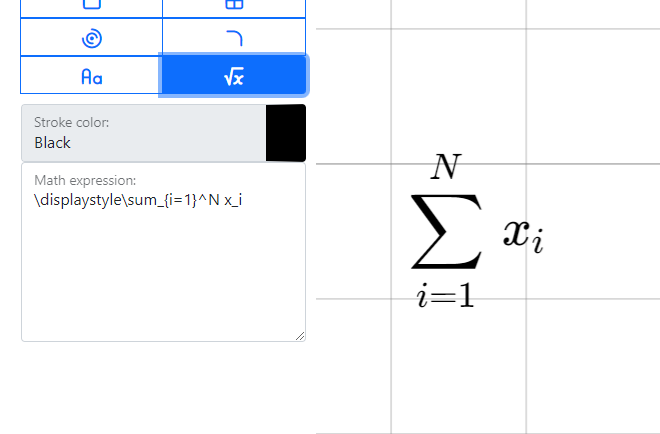
\includegraphics[width=0.75\textwidth]{images/math.png}
	\caption{Példa egy matematikai kifejezés megjelenítésére}
\end{figure}

A \textit{renderToCanvas} függvénnyel lehet a KaTeX által generált kifejezéseket a vászonra rakni, paraméterként meg kell adni a kirajzolandó kifejezést, magát a vásznat, mint kirajzolási hely, valamint a kifejezés pozícióját (az x és y koordinátát egyaránt).

\begin{lstlisting}[style=es6, morekeywords={document, P5, katex}]
let canvas = document.getElementById(P5.canvas.id);
katex.renderToCanvas(this.latex, canvas, 
    this.x + grid_density / 8, this.y - grid_density / 2.5, {
	    fontSize: 19.5
});
\end{lstlisting}

A \textit{TikZ} megoldás egyszerűbb, ott egy \textbackslash \textit{node} parancs paramétereként kell megadni a kifejezést matematikai módban.

\SubSubSection{Text osztály}

A \textit{Text} osztály szöveg vászonra helyezését teszi levetővé. Példányosítás ugyanúgy zajlik, mint a matematikai kifejezések esetében.

Annak ellenére, hogy a \textit{p5.js} rendelkezik olyan funkciókkal ezek "kirajzolása" szintén a KaTeX függvénykönyvtár segítségével történik, annyi eltéréssel, hogy a kirajzolandó szöveg megkapja a \textbackslash text\{\} paramétert, hogy ne érvényesüljön a matematikai mód.

\begin{lstlisting}[style=es6, morekeywords={document, P5, katex}]
let canvas = document.getElementById(P5.canvas.id);
katex.renderToCanvas(`\\text{${this.text}}`, canvas, 
    this.x + grid_density / 8, this.y - grid_density / 2.5, {
	    fontSize: 19.5
});
\end{lstlisting}

A \textit{TikZ} megoldás hasonlóan a \textbackslash \textit{node} parancs paramétereként kell megadni a szöveget.

\SubSection{Funkciók osztályai}

Itt a két funkció kerül bemutatásra, ami osztályba lett szedve a könnyebb elérés miatt. A funkciók jelentős része modulként szerepel az alkalmazásban, nem osztályokba csoportosítva.

\SubSubSection{Control osztály}

Ez az osztály felelős a vászon mozgatásáért és a nagyításért. Az osztályban eseménykezelők kerültek létrehozásra: kezelésre kerül az egér kattintása, húzása, felengedése valamint a görgetés. A vászon mozgatása szintén a "drag and drop" elvet követi.

Az eseménykezelők beállítása a \textit{p5.js} példányára, amely a \textit{sketch}-ben kerül létrehozásra:

\begin{lstlisting}[style=es6, morekeywords={P5, Control}]
P5.mousePressed = e => Control.mousePressed(e)
P5.mouseDragged = e => Control.mouseDragged(e);
P5.mouseReleased = e => Control.mouseReleased(e);
P5.mouseWheel = e => Control.zoomCanvas(e);
\end{lstlisting}

\SubSubSection{ColorPicker osztály}

Ez az osztály kezeli az alkalmazásban szereplő színválasztó megfelelő működését. Itt kerül kezelésre az adott színválasztó kiválasztása, a színpaletta megjelenítésé és eltüntetésé, az adott szín kijelölése. 

\begin{figure}[!h]
	\centering
	\label{fig:cp2}
	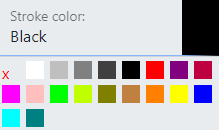
\includegraphics[]{images/colorpicker.png}
	\caption{Példa a színek kiválasztására}
\end{figure}

A színválasztó előredefiniált színek alapján dolgozik, ezek megegyeznek a \LaTeX\ által definiáltakkal:

\begin{lstlisting}[style=es6]
const COLOR = {
	NONE: "#E9ECEF", // for no stroke or fill color
	WHITE: "#FFFFFF",
	LIGHTGRAY: "#BFBFBF",
	GRAY: "#808080",
	DARKGRAY: "#404040",
	BLACK: "#000000",
	RED: "#FF0000",
	VIOLET: "#800080",
	PURPLE: "#BF0040",
	MAGENTA: "#FF00FF",
	PINK: "#FFBFBF",
	GREEN: "#00FF00",
	LIME: "#BFFF00",
	OLIVE: "#808000",
	BROWN: "#BF8040",
	ORANGE: "#FF8000",
	YELLOW: "#FFFF00",
	BLUE: "#0000FF",
	CYAN: "#00FFFF",
	TEAL: "#008080"
}
\end{lstlisting}

Azért ilyen formában kerülnek tárolásra a színkódok, mert a \textit{p5.js} tudja kezelni a hexadecimális színkódokat. A \textit{COLOR}-ra hivatkozva meg tudjuk adni a színeket. Például piros körvonal, és világosszürke kitöltés esetében:
\begin{lstlisting}[style=es6, morekeywords={P5, COLOR}]
P5.stroke(COLOR.RED);
P5.fill(COLOR.LIGHTGRAY);
\end{lstlisting}


\Chapter{Tesztelés}

A fejezetben be kell mutatni, hogy az elkészült alkalmazás hogyan használható.
(Az, hogy hogyan kell, hogy működjön, és hogy hogy lett elkészítve, az előző fejezetekben már megtörtént.)

Jellemzően az alábbi dolgok kerülhetnek ide.
\begin{itemize}
\item Tesztfuttatások. Le lehet írni a futási időket, memória és tárigényt.
\item Felhasználói kézikönyv jellegű leírás. Kifejezetten a végfelhasználó szempontjából lehet azt bemutatni, hogy mit hogy lehet majd használni.
\item Kutatás kapcsán ide főként táblázatok, görbék és egyéb részletes összesítések kerülhetnek.
\end{itemize}

\Chapter{Összefoglalás}

A szakdolgozatom célja egy olyan online grafikus szerkesztő létrehozása volt, amellyel \LaTeX-be visszailleszthető kód hozható létre. 

A dolgozat elkészítése közben alaposabban megismerhettem a Bootstrap 5 \cite{bootstrap} eszköztárral, a KaTeX \cite{katex}, és a \textit{p5.js} \cite{p5js} függvénykönyvtárak működését, előnyeit, hátrányait, és hiányosságait. Ha újra abban a helyzetben lennék, hogy válogatni kellene a könyvtárak közül, biztos vagyok benne, hogy ugyanúgy ezeket választanám. A különböző könyvtárak dokumentációja az online felületükön is elérhetők, interaktív példákkal illusztrálva a működésüket.

Véleményem szerint sikerült egy olyan webes alkalmazást létrehoznom, amely beleillik a mai modern weboldalakba. A célom az volt, hogy egy egyszerű, könnyen használható, azonban mégis funkciókban gazdag alkalmazás készüljön el. Az alkalmazás jelen formájában kiszolgálja egy átlag felhasználó igényeit: tud másolni, beilleszteni és törölni, lehet pontokat mozgatni, valamint meglévő ábrák tulajdonságait módosítani. A már kész ábrák visszatölthetők későbbi szerkesztésre.

A szoftverfejlesztésben még mindig rengeteg lehetőség és esély rejlik. Az alkalmazásom esetében az egyik, amit kiemelnék ezek közül a \LaTeX\ forráskód betöltése, ugyanis jelenleg minden elkészült ábrához tartozik egy kódolt karaktersorozat, amely tartalmazza az információkat, melyből az adott alakzat visszatölthető. Jelenleg a pontok mozgatása kissé körülményes tud lenni nagyobb és részletesebb ábrák esetében, illetve egy teljes alakzat mozgatásához az összes pontját ki kell jelölni. A pontok mozgatásánál jelenleg minden lerakott ábra összes pontja megjelenik, a jövőben célszerű lenne először egy kijelölésre leszűkítve megjeleníteni ezeket. Az alakzatok mozgatása esetében pedig célravezető, ha egy pont kijelölésével az elem összes pontja kiválasztásra kerül, amennyiben például \textit{ALT} billentyű lenyomása közben történik.

Abban egészen biztos vagyok, hogy a szakdolgozat elkészítése során szerzett rengeteg hasznos ismeretet alkalmazni tudom majd a jövőben is.

\clearpage

\addcontentsline{toc}{chapter}{Irodalomjegyzék}
\bibliographystyle{plain}
\bibliography{dolgozat.bib}

\newpage

\pagestyle{empty}

\noindent \textbf{\Large A mellékelt CD tartalma}

\vskip 1cm

\noindent A dolgozathoz tartozó melléklet a következőket tartalmazza:

\begin{itemize}
\item \texttt{thesis.pdf}: a dolgozat PDF formátumban
\item \texttt{manual.pdf}: a használati útmutató PDF formátumban
\item \texttt{thesis/}: a dolgozat \LaTeX\ forráskódját tartalmazó jegyzék
\item \texttt{editor/}: az elkészített szerkesztő jegyzéke
\end{itemize}

\vskip 0.5cm

\noindent
A szerkesztő futtatásához egy webszerver szükséges. Amennyiben nem áll rendelkezésre akkor egy \textit{Node.js} telepítése az egyik legegyszerűbb megoldás. Ez letölthető az alábbi linken:

\vskip 0.5cm
\noindent
\href{https://nodejs.org/en/download/}{\texttt{https://nodejs.org/en/download/}}

\vskip 0.5cm
\noindent
A \textit{http-server} telepítése:

\begin{lstlisting}[language=bash]
>   npm install --global http-server
\end{lstlisting}

\vskip 0.5cm

\noindent
Az alkalmazás elindításához ezenkívül egy parancssorra lesz szükség:

\begin{lstlisting}[language=bash]
>   http-server ./editor/
\end{lstlisting}

\vskip 0.5cm

\noindent
A parancs kiadása után már el is érhető al alkalmazás, jelen esetben a \textit{8080}-as port alatt:

\begin{lstlisting}[language=bash, alsoletter=0123456789, morekeywords={visible, none, disabled, seconds, 3600, 120, 8080}]
>   http-server ./editor/
Starting up http-server, serving ./editor/

http-server version: 14.0.0

http-server settings:
CORS: disabled
Cache: 3600 seconds
Connection Timeout: 120 seconds
Directory Listings: visible
AutoIndex: visible
Serve GZIP Files: false
Serve Brotli Files: false
Default File Extension: none

Available on:
http://192.168.0.2:8080
http://127.0.0.1:8080
	
Hit CTRL-C to stop the server
\end{lstlisting}


\end{document}
